% $Id: template.tex 11 2007-04-03 22:25:53Z jpeltier $

\documentclass{vgtc}                          % final (conference style)
%\documentclass[review]{vgtc}                 % review
%\documentclass[widereview]{vgtc}             % wide-spaced review
%\documentclass[preprint]{vgtc}               % preprint
%\documentclass[electronic]{vgtc}             % electronic version

%% Uncomment one of the lines above depending on where your paper is
%% in the conference process. ``review'' and ``widereview'' are for review
%% submission, ``preprint'' is for pre-publication, and the final version
%% doesn't use a specific qualifier. Further, ``electronic'' includes
%% hyperreferences for more convenient online viewing.

%% Please use one of the ``review'' options in combination with the
%% assigned online id (see below) ONLY if your paper uses a double blind
%% review process. Some conferences, like IEEE Vis and InfoVis, have NOT
%% in the past.

%% Figures should be in CMYK or Grey scale format, otherwise, colour 
%% shifting may occur during the printing process.

%% These few lines make a distinction between latex and pdflatex calls and they
%% bring in essential packages for graphics and font handling.
%% Note that due to the \DeclareGraphicsExtensions{} call it is no longer necessary
%% to provide the the path and extension of a graphics file:
%% \includegraphics{diamondrule} is completely sufficient.
%%
\ifpdf%                                % if we use pdflatex
  \pdfoutput=1\relax                   % create PDFs from pdfLaTeX
  \pdfcompresslevel=9                  % PDF Compression
  \pdfoptionpdfminorversion=7          % create PDF 1.7
  \ExecuteOptions{pdftex}
  \usepackage{graphicx}                % allow us to embed graphics files
  \DeclareGraphicsExtensions{.pdf,.png,.jpg,.jpeg} % for pdflatex we expect .pdf, .png, or .jpg files
\else%                                 % else we use pure latex
  \ExecuteOptions{dvips}
  \usepackage{graphicx}                % allow us to embed graphics files
  \DeclareGraphicsExtensions{.eps}     % for pure latex we expect eps files
\fi%

%% it is recomended to use ``\autoref{sec:bla}'' instead of ``Fig.~\ref{sec:bla}''
\graphicspath{{figures/}{pictures/}{images/}{./}} % where to search for the images

\usepackage{microtype}                 % use micro-typography (slightly more compact, better to read)
\PassOptionsToPackage{warn}{textcomp}  % to address font issues with \textrightarrow
\usepackage{textcomp}                  % use better special symbols
\usepackage{mathptmx}                  % use matching math font
\usepackage{times}                     % we use Times as the main font
\renewcommand*\ttdefault{txtt}         % a nicer typewriter font
\usepackage{cite}                      % needed to automatically sort the references
\usepackage{tabu}                      % only used for the table example
\usepackage{booktabs}                  % only used for the table example
%% We encourage the use of mathptmx for consistent usage of times font
%% throughout the proceedings. However, if you encounter conflicts
%% with other math-related packages, you may want to disable it.


%% If you are submitting a paper to a conference for review with a double
%% blind reviewing process, please replace the value ``0'' below with your
%% OnlineID. Otherwise, you may safely leave it at ``0''.
\onlineid{0}

%% declare the category of your paper, only shown in review mode
\vgtccategory{Research}

%% allow for this line if you want the electronic option to work properly
\vgtcinsertpkg

%% In preprint mode you may define your own headline.
%\preprinttext{To appear in an IEEE VGTC sponsored conference.}

%% Paper title.

\title{User Evaluation of Group-in-a-box Variants}

%% This is how authors are specified in the conference style

%% Author and Affiliation (single author).
%%\author{Roy G. Biv\thanks{e-mail: roy.g.biv@aol.com}}
%%\affiliation{\scriptsize Allied Widgets Research}

%% Author and Affiliation (multiple authors with single affiliations).
%%\author{Roy G. Biv\thanks{e-mail: roy.g.biv@aol.com} %
%%\and Ed Grimley\thanks{e-mail:ed.grimley@aol.com} %
%%\and Martha Stewart\thanks{e-mail:martha.stewart@marthastewart.com}}
%%\affiliation{\scriptsize Martha Stewart Enterprises \\ Microsoft Research}

%% Author and Affiliation (multiple authors with multiple affiliations)
\author{Nozomi Aoyama\thanks{e-mail: aoyama.nozomi.37x@st.kyoto-u.ac.jp}\\ %
        \scriptsize Kyoto University %
\and Yosuke Onoue\thanks{e-mail: onoue.yousuke@nihon-u.ac.jp}\\ %
     \scriptsize Nihon University %
\and Yuki Ueno\thanks{e-mail: ueno.yuki.78x@st.kyoto-u.ac.jp}\\ %
     % \parbox{1.4in}{
     \scriptsize \centering Kyoto University
\and Hiroaki Natsukawa\thanks{e-mail: natsukawa.hiroaki.3u@kyoto-u.ac.jp}\\ %
     \scriptsize Kyoto University
\and Koji Koyamada\thanks{e-mail: koyamada.koji.3w@kyoto-u.ac.jp}\\ %
     \scriptsize Kyoto University}

%% A teaser figure can be included as follows, but is not recommended since
%% the space is now taken up by a full width abstract.
%\teaser{
%  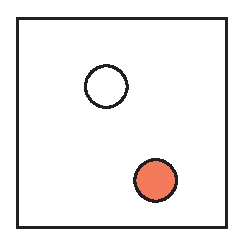
\includegraphics[width=1.5in]{sample.eps}
%  \caption{Lookit! Lookit!}
%}

%% Abstract section.
\abstract{
Group in a box (GIB) is a graph-drawing method designed for visualizing the group structure of graphs.
GIB allows the group sizes and both the inter- and intra-group structures to be viewed simultaneously.
Several GIB variants have been proposed to realize each design
goal.
However, their advantages and disadvantages from the perspective of human cognition have not been studied.
Herein, we conducted a user evaluation, including eye-tracking analysis, of four GIB variants.
As a result, we found the superiority of FD-GIB and TR-GIB in many tasks from the evaluation, .
Although ST-GIB did not give a bad result, it was inferior in terms of the link readiability.
The eye-tracking analysis provided some clues as to why these results were generated and what element affect the experiment result.
We also provide a website that make the four GIB layout available in the form of a bitmap or a svg imagefile.
This study will encourage effective use of GIB to promote  analysis of network diagrams such as social network or web graphs.
} % end of abstract

%% ACM Computing Classification System (CCS). 
%% See <http://www.acm.org/about/class> for details.
%% We recommend the 2012 system <http://www.acm.org/about/class/class/2012>
%% For the 2012 system use the ``\CCScatTwelve'' which command takes four arguments.
%% The 1998 system <http://www.acm.org/about/class/class/2012> is still possible
%% For the 1998 system use the ``\CCScat'' which command takes four arguments.
%% In both cases the last two arguments (1998) or last three (2012) can be empty.

\CCScatlist{
  \CCScatTwelve{Human-centered computing}{Visu\-al\-iza\-tion}{Visu\-al\-iza\-tion techniques}{Treemaps};
  \CCScatTwelve{Human-centered computing}{Visu\-al\-iza\-tion}{Visualization design and evaluation methods}{}
}

%\CCScatlist{
  %\CCScat{H.5.2}{User Interfaces}{User Interfaces}{Graphical user interfaces (GUI)}{};
  %\CCScat{H.5.m}{Information Interfaces and Presentation}{Miscellaneous}{}{}
%}

%% Copyright space is enabled by default as required by guidelines.
%% It is disabled by the 'review' option or via the following command:
% \nocopyrightspace

%%%%%%%%%%%%%%%%%%%%%%%%%%%%%%%%%%%%%%%%%%%%%%%%%%%%%%%%%%%%%%%%
%%%%%%%%%%%%%%%%%%%%%% START OF THE PAPER %%%%%%%%%%%%%%%%%%%%%%
%%%%%%%%%%%%%%%%%%%%%%%%%%%%%%%%%%%%%%%%%%%%%%%%%%%%%%%%%%%%%%%%%

\begin{document}

%% The ``\maketitle'' command must be the first command after the
%% ``\begin{document}'' command. It prepares and prints the title block.

%% the only exception to this rule is the \firstsection command
\firstsection{Introduction}

\maketitle

%% \section{Introduction} %for journal use above \firstsection{..} instead
In the area of graph drawing, numerous methods have been proposed, each aiming at a different visualization goal.
Some of the methods are designed for the analysis of real-world graph data, such as social networks and web graphs.
They are often characterized as being so-called complex networks \cite{Newman:2010:NI:1809753}, a feature of which is their community structure \cite{girvan2002community,newman2004detecting}.
A network with a community structure contains certain groups and nodes which belong to the groups.
Additionally, this kind of data often provides several nodes and have dense within-group edges and sparse between-group edges.
For example, consider a Twitter network data, it has users as nodes and edges connecting couples of users representing one replies to or mentions the other.
Users can be divided to some groups in such a network using the whole topology of the graph or its feature.
When a network become larger and with higher density, it can be more challenging for an observer to understand this network data because of the high number of nodes, edges, and groups resulting in visual clutter.
To analyze the real-world data, an effective visualization technique for understanding the group structure of the network is essential.

There are various methods to group related nodes in a network based on a feature of that such as the topology, some attributes the nodes have, or the combination of them \cite{clauset2004finding,wakita2007finding,lloyd1982least,navlakha2009finding}.
A topological method generate groups so that the relationships among nodes in a single group are stronger than those beween nodes in different groups.
The latter method take some common attributes to the nodes. For example in the case of Twitter network, there are user's geographical location, religion, and interests.
General methods to illustrate these groups visually discriminate them by colour or shape of nodes, which is not effective way to make it easy to understand when a network is large.

Group in a box (GIB) is a graph-drawing method designed for a network in which a node belong to a group, and visualize the group structures in graphs.
GIB arranges all nodes in a group into a box with an area proportional to the number of nodes in the group so that each group are visualized separatedly.
It then lays groups inside their boxes with a force-directed, circle, grid or other available layout.
Using a GIB layout enables the simultaneous visualization of group structures, intra-group relationships, inter-group relationships and the sizes of the groups in a graph.
This method supports data scalability, and can work in large scale networks.
It is especially expected that placing groups in individual boxes helps understand intra-group information much more than without boxes.
There are several variants of GIB layout \cite{rodrigues2011group,chaturvedi2014group,onoue2017optimal} as shown in Fig.\ref{GIB-examples}, and each of them aims different purpose originally.
Although a few computational experiments \cite{chaturvedi2014group,onoue2017optimal} have evaluated these GIB variants, they have not been evaluated through user experiments to the best of our knowledge.
Some network measures are used in such computational experiments(e.g., the number of edge crossings) known to affect the readability of a graph drawing \cite{468391,purchase1997aesthetic,purchase1998performance,purchase2002empirical}, but other elements related to readability in GIB visualizations make user experiments important.

Herein, we aim to ascertain which GIB variant is the most effective.
We report on the evaluation of four GIB variants, namely ST-GIB, CD-GIB, FD-GIB, and TR-GIB, with four types of user tasks. The tasks are designed based on the studies by Vehlow et al.
\cite{Vehlow2017VisualizingGS} and Saket et al. \cite{saket2014group} to view each layout's features from various perspectives.
We measure the task accuracy and completion time for each task.
We also collect the eye-tracking data of participants during the tasks.

Eye-tracking is a technique for recording gaze data and often used user experiments in the field of visualization and human-computer interaction science.
It is useful for analyzing tasks in this case because the gaze data of participants can give us some insights into why the layouts affect the results \cite{andrienko2012visual,duchowski2007eye,kurzhals2014evaluating}.
In addition to the accuracy and completion time of tasks, we also analyze the eye-tracking data to reveal why one layout is better than the other layout.
Specifically, we focus on revealing what element in a layout makes it easy or difficult to solve tasks.

One of our main contribution is to evaluate 4 GIB layouts and find the best GIB.
We assume that each GIB has its advantage and disadvantage, so we aim to evaluate these GIB variants with 4 tasks and verify which task is significantly superior in each task.
We also provide some evidence for the result with eye tracking with an aim to clarify what element in a visualization affect the result.
In addition, we make it possible to avail these 4 GIB layout for public. Our website (http://gib.jgs-hd.com) provide GIB image, as well as further analysis of the network. It can help researchers analyze their network data and possibly give them new findings.

\begin{figure*}[t]
  \begin{center}
    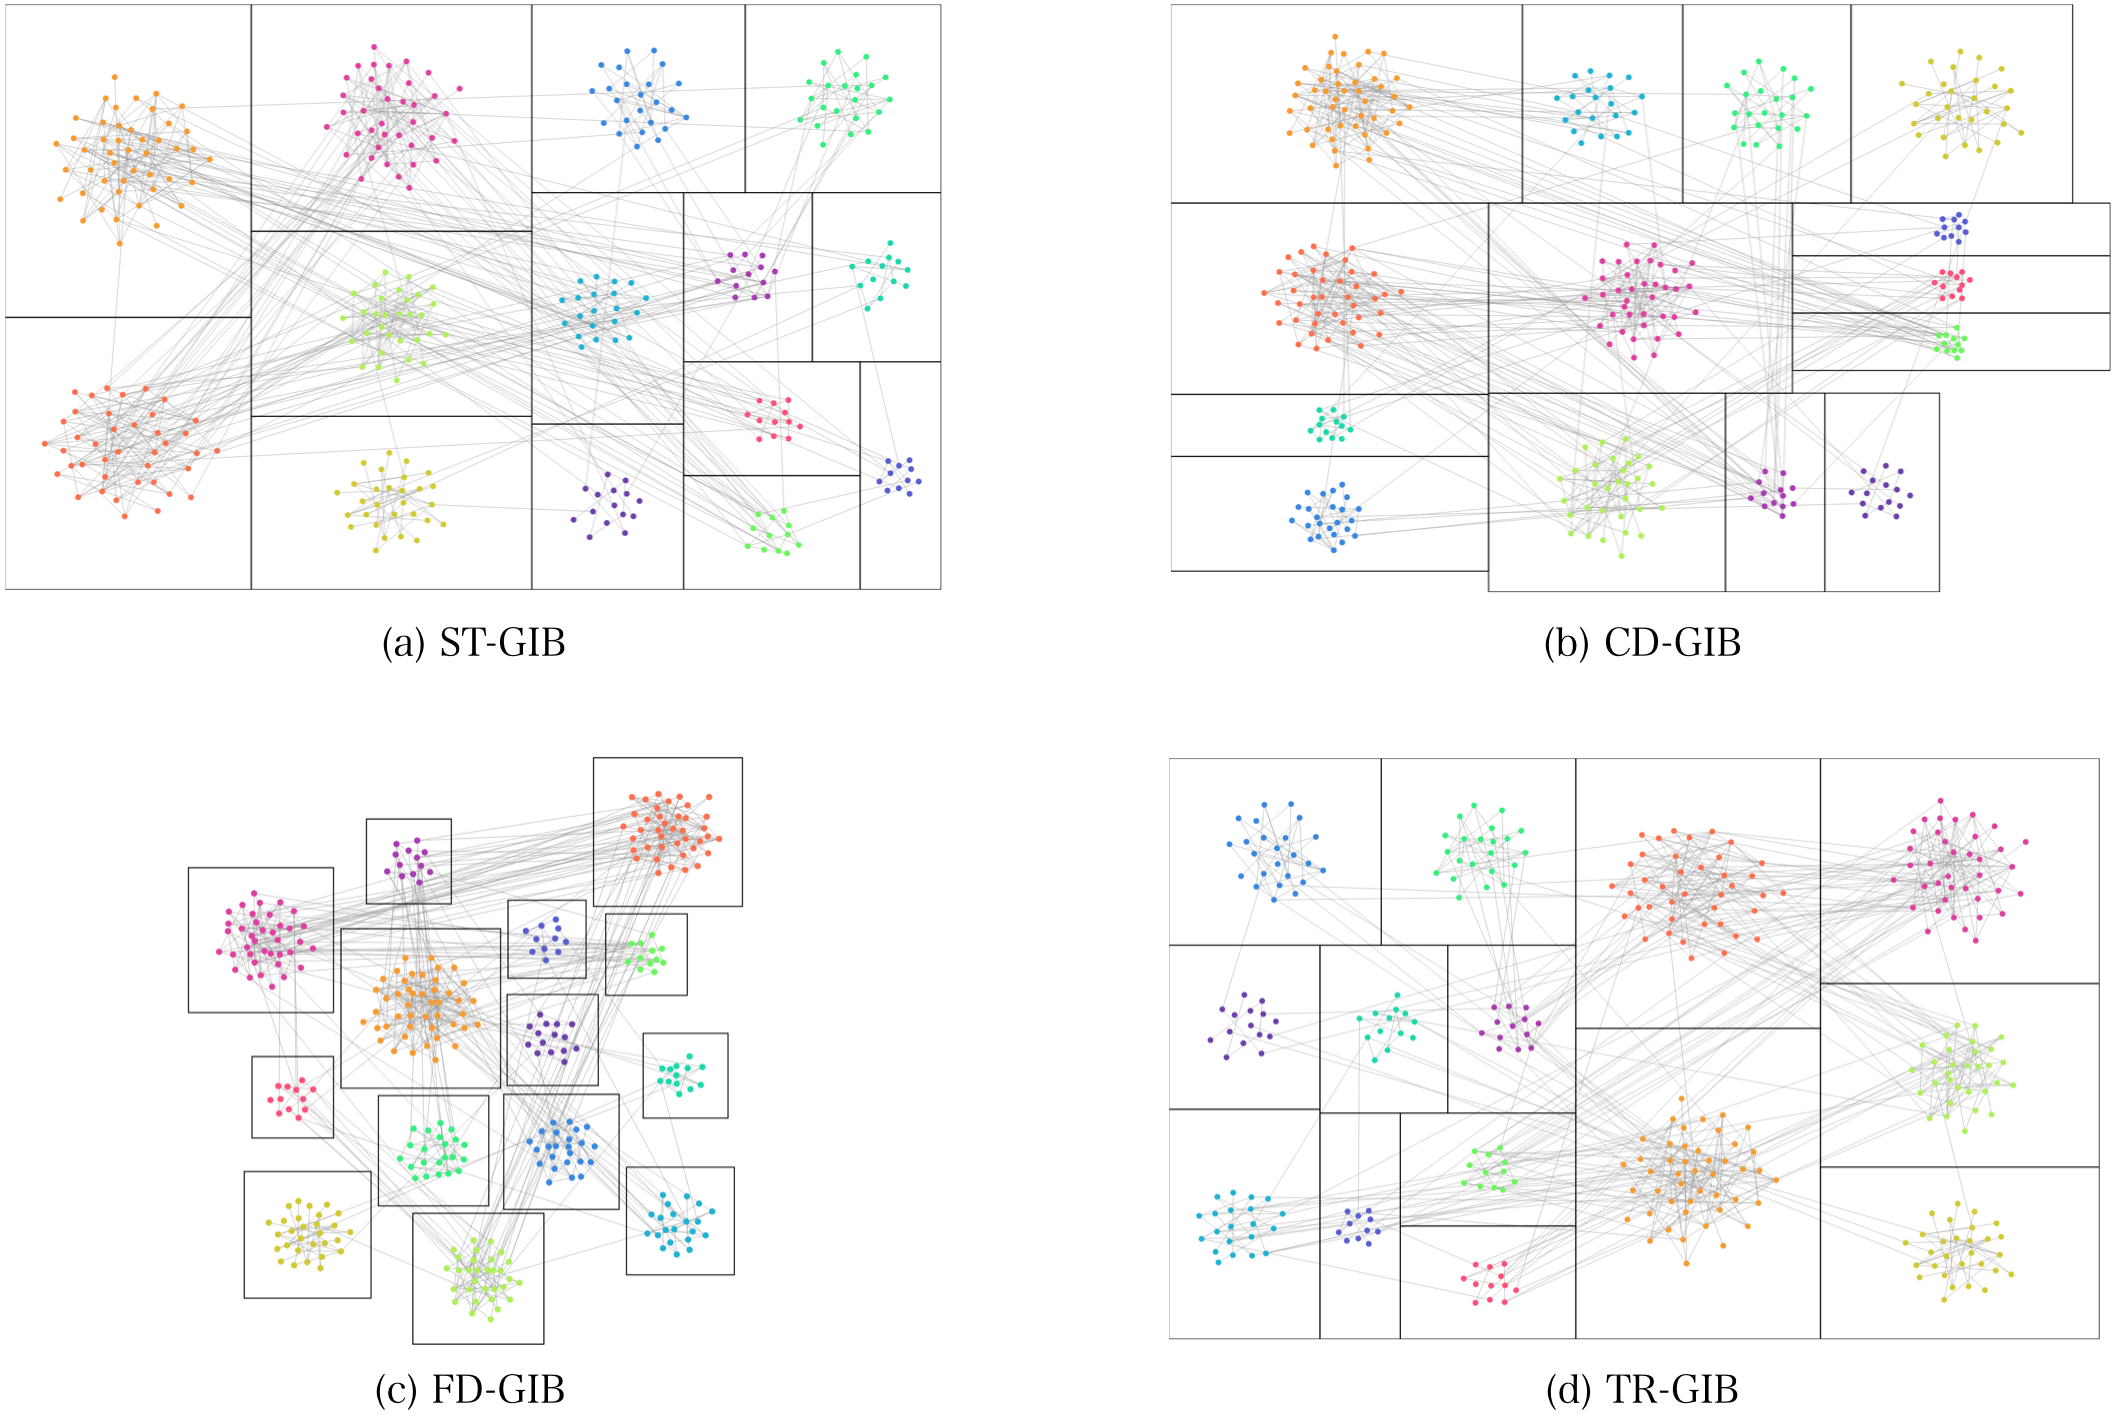
\includegraphics[width=1\textwidth]{pictures/examples.png}
    \caption{Examples of group-in-a-box (GIB) layouts. Four GIB layout look different but the origin data is the same.}
    \label{GIB-examples}
  \end{center}
\end{figure*}

%
\section{Related Work}
%
\subsection{Graph Drawing method for group structure}
A purpose of a graph drawing method is to design a layout diagram for complex network. Thomas et al. proposed a method using force-directed placement, in which consider attractive and repulsive force to produce an optimal equilibrium \cite{fruchterman1991graph}. This force-directed method has been widely used and applied to various forms. There are several other approaches \cite{harel2000fast,koren2003drawing,hachul2004drawing,article} for visualizing complex network. Although these general visualizations takes network structure in to account, they do not visualize the complexity of group structure explicitly, so are often challenging for the understanding of a clustered graph. 

On the other hand, the recent popularity of the network visualization has developed some techniques designed for the network with group structure. In large scale network data, the importance of community detection is known and several approach, often based on force-directed layout, have been invented. One traditional method to illustrate the group structure of a graph is varying the colour \cite{mcpherson2005discovering} or the shape of node, but often not effective in the real world network.

Vehlow et al. provides an survey paper about visualization of group structure in graphs \cite{Vehlow2017VisualizingGS}.
They describes a taxonomy of such visualization and also that of tasks used in user-study experiments for them.
The visualization taxonomy is clussified by two ways, vertex group visualization and vertex group structure.
The former one represent how the nodes are grouped, and the categories are namely visual node attributes, juxtaposed, superimposed and embedded.
The latter depends on whether a network can be characterized by either or both of group overlapping and hierarchy of the structure or not.
A node in a network with group overlapping can belong to multiple groups at the same time.
A hierarchical network has some hierarchical structure among groups.
They introduced some visualizations designed for a network with group structure at each category in the taxonomy.

The GIB, Group-In-a-Box, layout is also a visualization for group structure categorized as with no group overlapping presented in \cite{rodrigues2011group,chaturvedi2014group,onoue2017optimal}. There are 4 major variants of GIB which we tackle in this research, ST-GIB, CD-GIB, FD-GIB, FD-GIB. This data-scalable layout have an advantage of visualizing each groups clearly seperated, which allow to observe a relationship between two node in the same group easily. It can also provide the information of group size quickly as a form of the rectangular's area.
This categorized as a method of superimposed visualization and for the network without group overlapping in Vehlow's taxonomy, and ST-GIB and TR-GIB can be applied for a network with hierarchical structure.
An example of network data in which GIB is effective is a Twitter data with some groups defined as the users location, because the location can not make an overlap.

In terms of the evaluation of GIB, Chaturvedi et al. \cite{chaturvedi2014group} compared three kind of GIB, namely ST-GIB, CD-GIB and FD-GIB, by computing some measures: edge-box overlap, percent screen space wasted, execution time and mean group-box aspect ratio.
They also provides some case studies.
They observed strong differences of the computational measures among the three layouts, especially FD-GIB is good at reducing the number of edge-box overlaps but not at saving screen space.

Although this kind of evaluation is effective to choose one layout for specific purpose, but it's not enough because there are hidden factors which have influence at the readability. One effective way to evaluate them including such hidden factors is user study, and with using multiple tasks more spherical discussion might be done. This time we focus on four GIB layouts, ST-GIB, CD-GIB, FD-GIB and TR-GIB, and aims to ascertain which layout is the best in our user study.

\subsection{Evaluation with Eye tracking}
Several studies have done evaluations of visualization with eye tracking \cite{burch2011evaluation,pohl2009comparing,netzel2014comparative,jianu2014display,7539393}. An eye-track system can collect the gaze data, and has been widely used to measure visual attention of the participants, and often to analyze how well participants perform at user study. It is known that researchers can elicit a clue to find why a visualization is better than the others by analyzing gaze data.

Burch et al. evaluated three variants of tree diagram, traditional, orthogonal, and radial tree with eye tracking \cite{burch2011evaluation}. They imposed participants a task to find the least common ancestor of a set of given nodes. They collected gaze data as well as the task accuracy and the completion time, and analyzed it using some tequnique designed for the analysis of gaze data, such as trajectory map, heat map, and gaze flow between a pair of AOI (area of interest). This eye-track analysis gave them an insight about why some differences were made in the task result, specifically cross-check trajectories in a layout with the least accuracy.

There are some studies providing guidlines about visual analytics \cite{andrienko2012visual,kurzhals2014evaluating,duchowski2007eye}.
Eye-track data is often enormous and quite hard to analyze. Therefore this spatio-temporal gaze data need some specific methodologies for the analysis.
For an effective and meaningful analytics, it is important to know what kind of methods are most appropriate for employing, and these studies can give reseachers some hints about it.

We collect gaze data during the tasks in order to reveal what element in a visualization affect the performance. We suppose this study become more meaningful by referring these analysis guidelines.


\section{GIB Layouts}
%{}
In this section, we describe the four evaluated GIB variants, namely ST-GIB, CD-GIB, FD-GIB, and TR-GIB, the examples of which are shown in Fig.~\ref{GIB-examples}.
Each graph in this figure has a different layout of GIB, but each use the same data as a origin network data.
We use force-directed layout to draw network in a box in this figure, but other methods can be applied.

\subsection{ST-GIB}
Squarified treemap GIB (ST-GIB) (Fig.~\ref{GIB-examples}(a)) is a layout based on squarified treemaps by Bruls et al. \cite{bruls2000squarified} and proposed by Rodrigues et al. \cite{rodrigues2011group}.
Bruls' method was originally for treemapping, which is a visualization method that takes rectangular regions and numerical columns as inputs to divide a region into tiles with areas proportional to their values \cite{shneiderman1992tree}.

In ST-GIB, the groups are taken as vertices in treemaps and shown in the shape of tiles that have nodes belonging to its group in it.
The treemap algorithm facilitates a space-filling arrangement with low-aspect-ratio boxes, which is important for analyzing the rectangle content \cite{bruls2000squarified}.
However, the ST-GIB layout uses only the squarified treemap algorithm to arrange group networks in rectangles, so it does not consider the relationships among nodes when the tiles are placed.
This problem causes link overlaps, which considerably hamper the understanding of networks \cite{468391,purchase1997aesthetic,purchase1998performance,purchase2002empirical}.
To arrange tiles using this method, we utilized the Python library squarify (https://github.com/laserson/squarify), which employs Bruls' algorithm. This method arrange the boxes in the order of box size, which might make it easy to compare the group size.

\subsection{CD-GIB}
Chaturvedi et al. \cite{chaturvedi2014group} presented a croissant-and-doughnut GIB (CD-GIB) (Fig.~\ref{GIB-examples}(b)).
They developed this layout to improve ST-GIB to be able to consider network information connecting a node to another of a different group.
Concretely, they worked on arranging tiles based on G-degree and G-skewness.
A group's G-degree is defined as the number of other groups it is connected to, and G-skewness refers to the fraction of nodes present in the two most-connected groups (groups with the highest G-degree).
One layout is then chosen from croissant-GIB, doughnut-GIB, or ST-GIB according to the total number of groups and the G-skewness.
Chaturvedi et al. defined the criteria for using the three methods properly, which are also used by us.

Croissant-GIB, one of the layouts Chaturvedi et al. proposed, assign the most connected box which has the highest G-degree at the center-top of the screen. The other boxes are set so that they surround the most connected box, resulting in a shape of a croissant. another layout, doughnut-GIB, assign the most connected box at the center with other boxes surrounding it, so the whole boxes look like a doughnut.

In both layouts, the most connected is placed close to the center to allow these methods to account for links among groups, so we expect better readability than that achieved with ST-GIB because of fewer edge crossings \cite{468391,purchase1997aesthetic,purchase1998performance,purchase2002empirical}.
However, the aspect ratio of a box tends to be worse, which can affect the rectangle content's capability of being analyzed \cite{bruls2000squarified}.

\subsection{FD-GIB}
Chaturvedi et al. \cite{chaturvedi2014group} also provided the FD-GIB layout (Fig.~\ref{GIB-examples}(c)).
%This approach explicitly shows the inter-group relationships.
The group boxes are arranged using a force-directed layout run on the whole network, where the vertices represent entire groups and the edges between them show the links between groups.
They then draw the group boxes on this initial layout centered at the group node's position.
This layout can cause group overlaps, which are removed using the PRISM method \cite{gansner2008efficient}; we use this method to eliminate all overlaps.

Chaturvedi et al. used the Harel--Koren fast multiscale layout \cite{harel2002graph} to arrange the rectangles in FD-GIB, but we use the D3.js force simulation (https://d3js.org/) because it is easy to obtain and produce good results.
However, as reported by Chaturvedi et al. \cite{chaturvedi2014group}, according to the experimental evaluations of several layout algorithms performed by Hachul et al. \cite{Hachul:2005:ECF:2102325.2102348,Hachul2007LargeGraphLA}, there are several good choices, such as the high-dimensional embedding approach \cite{harel2002graph} or the algebraic multi-grid method \cite{koren2003drawing}.

This layout has the benefit of showing the aggregate topology clearly, but it wastes more screen space.
The area of each group must be smaller than those of the others, so it is expected more difficult to see the relationships in a single group.
However, this layout can maintain a unit box aspect ratio, so we expect participants to easily recognize the size difference between boxes.

\subsection{TR-GIB}
Onoue et al. developed TR-GIB to minimize the weighed sum of distances between groups by reordering the sibling nodes in ST-GIB \cite{onoue2017optimal}.
An example of this is shown in Fig.~\ref{GIB-examples}(d).
This method looks similar to ST-GIB, but the tiles are reordered.
Treemaps, e.g., ST-GIB, have a tree-like structure, so vertices with the same depth in it can be reordered.
This layout aims to reduce the sum of the link distances, which results in less edge crossings that cause a misunderstanding.
The coordinates of this layout can be obtained by reordering those of the ST-GIB layout to minimize the proximity.
Specifically, the sum of the distances between two groups is weighted according to the number of edges between the two groups and this sum is taken as the group proximity.

This layout has the minimized group proximity, so the edge length is shortened, which leads to edge crossings lesser than those with ST-GIB.
We expect this layout to have the advantages of ST-GIB (i.e., good aspect ratio and screen efficiency) and the advantage of less edge overlaps.

\section{Data for Experiment}

\subsection{Data and Layout Generation}
\label{layout}

We used random data for these experiments, generated by a procedure similar to that used by Onoue et al. \cite{onoue2017optimal}.
Each graph consists of multiple groups with some strong edge connections between certain group pairs like real-world data.
There are two differences between this method and that proposed by Onoue et al. The first is the way of setting the number of groups randomly from a normal distribution with $m_{mean}$ and $m_{stdev}$ ranging from $m_{min}$ and $m_{max}$.
The second is that we determine the number of vertices in a vertex set $V_i$, which we determine based on the random numbers from a normal distribution with $v_{mean}$, $v_{stdev}$, and a minimum of $v_{min}$.
We calibrated the graph generation parameters listed in Table~\ref{params} to bring our data closer to the actual Twitter data reported by Chaturvedi et al. \cite{chaturvedi2014group}.
We set these parameters through several processes.
First, we calibrated them to make the numbers of groups, nodes, and links correspond to those reported by Chaturvedi et al.
However, this yielded more nodes and links than we could interpret, so we reduced them by multiplying $v_{mean}$ and $v_{stdev}$ by 0.4 and $p_{in}$, $p_{bridge}$, and $p_{out}$ by 0.3.
In this way, we obtained the graphs shown in Fig.~\ref{GIB-examples}.

\begin{table}[h]
  \begin{center}
  \caption{Parameters used for data generation}
    \begin{tabular}{|c|c|c|c|c|c|} \hline
      $m_{mean}$ & $m_{stdev}$ & $m_{min}$ & $m_{max}$ & $V_{mean}$ & $V_{stdev}$ \\ \hline 
      11.4 & 5.4 & 6 & 11 & 21.0 & 14.12 \\ \hline
    \end{tabular}
    \begin{tabular}{|c|c|c|c|c|} \hline
      $V_{min}$ & $p_{in}$ & $p_{group}$ & $p_{bridge}$ & $p_{out}$ \\ \hline
      4 & 0.0858 & 0.06 & 0.015 & 0.0006 \\ \hline
    \end{tabular}
  \end{center}
  \label{params}
\end{table}

After generating the data, we applied the four layouts to them separately, thereby obtaining the tile arrangements.
The four targeted layouts arrange only boxes, so we had to determine the node coordinates in a box.
Although there are many ways to place the nodes in a box, we used the force-directed layout.
This method is widely used in graph drawing wherein the nodes are subjected to repulsive between-node forces, attractive forces between adjacent nodes, and gravity from the center of the group tile to which they belong.
Although the layout inside the box certainly affects the results of tasks, force layout is known to reduce edge crossing, and we supposed that this layout is suitable.
However, another experiment with other layout will be also interesting.

We used straight lines for edges.
Other than straight lines, there are options such as edge bundling.
A graph srawing with straight lines become complex and edge bundling is effective when there too many edges.
However, as an advantage of a straight line, it can directory represent a relationship between two nodes, and we can more easily discriminate a specific edge from the others than a bundled line.
We suppose a situation that GIB layouts let reseachers further analysis with themselves where every relationship should be shown clearly, so we selected straight lines.

\subsection{Generated Layouts}
\label{computation}

There are various known metrics that can affect the readability of graph drawing.
As a pilot study, we computed three measures to obtain insights into the user study, namely the number of edge crossings, uniform edge length, the ratio of screen space wasted, and the mean group aspect ratio.
We chose these four metrics mainly with reference to those used by Chaturvedi et al. \cite{chaturvedi2014group}, although we used edge crossings rather than their edge box overlap.
For visualizing an inter-edge, they draw a bundled edge, resulting in the use of edge box overlap as a measure.
As mentioned in section \ref{layout}, we utilized straight lines for the representation of inter-links, therefore we can calculate the number of edge crossings, which can tell us the readability of a graph more directly.
We describe these metrics in detail below.

\begin{itemize}
\item {\bf Edge Crossings}

This metric is the total number of edge crossings, and known to reduce the readability of graph drawing and should therefore be small.
In particular, a long inter-edge can overlap with many other inter-edges and intra-edges of boxes on the edge's way.
We applied the same force-directed layout to all boxes to measure the number of interrupting factors for our data, as generated in Section~\ref{layout}.

\item {\bf Uniform Edge Length}

A uniform edge length is a measure representing to what extent the lengths of edges in a graph are uniform.
A survey paper of Gibson et al. explaiend this measure as an index for a regular structure that prevents the graph becoming distorted \cite{doi:10.1177/1473871612455749}.
We compute the variance of edge length in each graph as uniform edge length.
Therefore, the small variance means there are high uniformity in the length of the edge in a graph, which is known to lead high readability.

\item {\bf Parcentage of Screen Space Wasted}

A two-dimensional screen space-filling layout has the potential to be comprehensible \cite{shneiderman1992tree}.
In GIB, more efficient screen space causes boxes to become bigger and each network to be drawn with more screen space.
When screen space is limited, links can be too short to interpret and networks can become visually unappealing.
For effective visualization, screen space should not be wasted.

\item {\bf Mean Group Box Aspect Ratio}

Bruls et al. emphasize that rectangles that are more square-like have advantages such as screen efficiency, easier comparison of box size, and accuracy of presentation \cite{bruls2000squarified}.
They also note that thin rectangles cause aliasing errors, whereas square items are easier to detect and point at.
Because we use force-directed layouts that depend on the gravity from the center of the box, the network nodes tend to be arranged spherically, thereby yielding a good aspect ratio close to unity.

% This ratio is described as
% \begin{center}
% Mean Group-Box Aspect Ratio $= \frac{\sum_{i=1}^{N} a_i}{N} $
% \end{center}
% where $a_i$ is aspect ratio of the $i$th group and N is the total number of groups.
\end{itemize}

\begin{figure}[h]
  \begin{center}
    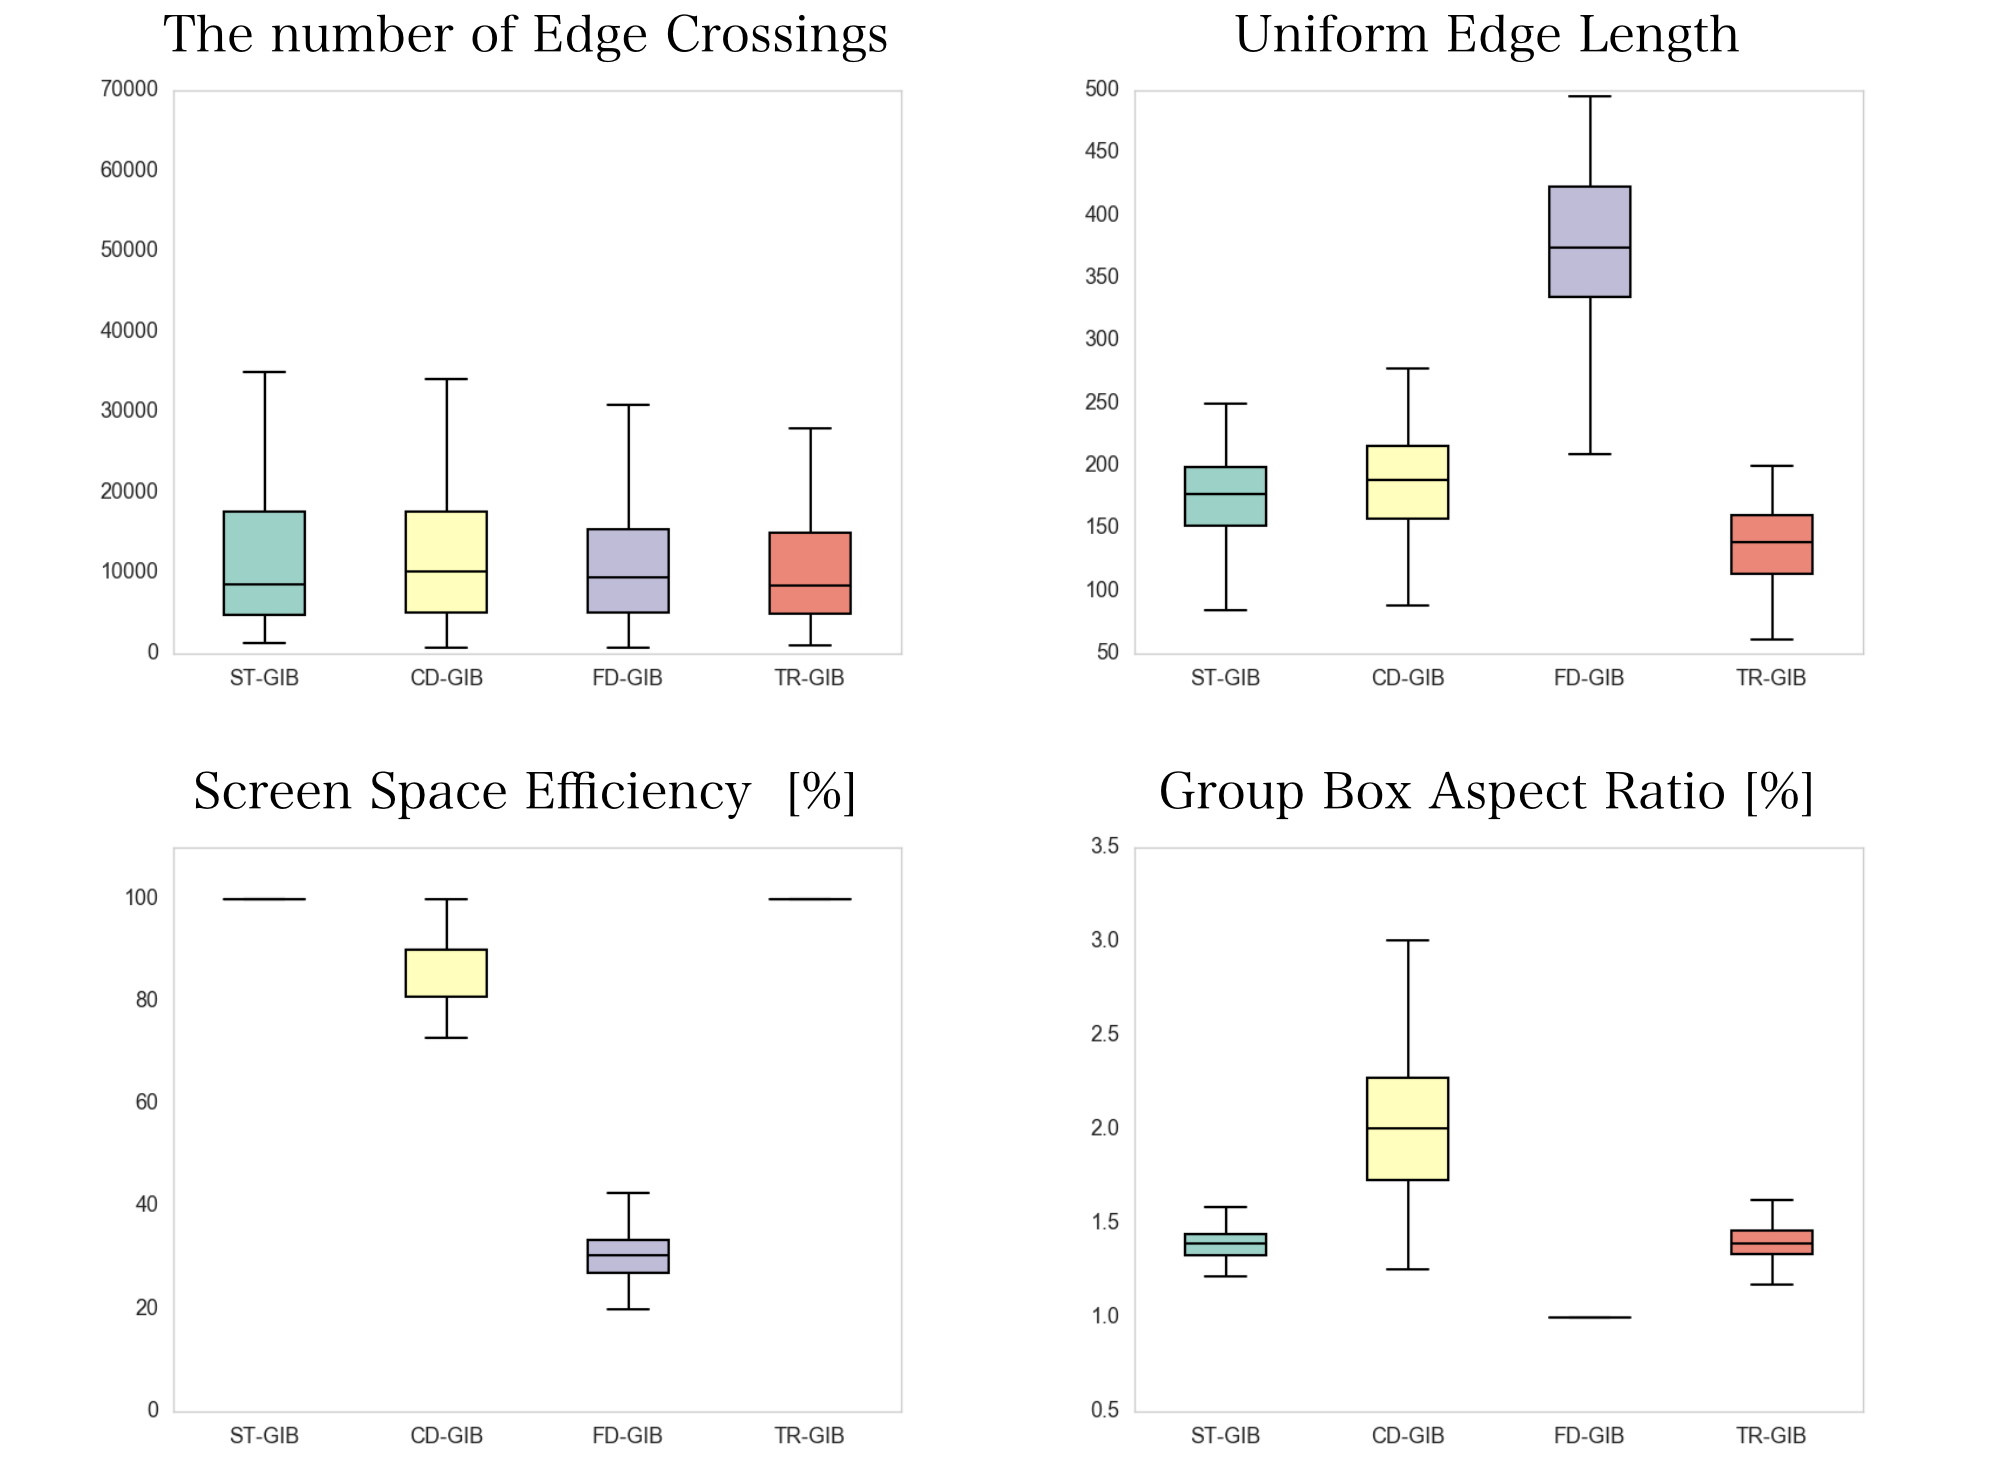
\includegraphics[width=0.48\textwidth]{pictures/computation.png}
    \caption{Computation result}
    \label{comp-result}
  \end{center}
\end{figure}

Fig.~\ref{comp-result} summarizes the calculation results.
In graph drawing, we demand fewer edge overlaps, lower aspect ratio,less wastage of screen space and small uniform edge length.
The results show that TR-GIB had the fewest edge crossings.
Additionally, TR-GIB achieved the best result and the FD-GIB was the worst in the uniform edge lendth, thereby indicating that TR-GIB is the most effective layout for reducing edge overlaps.

Regarding the ratio of wastage of screen space, it was low for ST-GIB and TR-GIB, followed by CD-GIB, as summarized in Table~\ref{comp-result}.
Furthermore, FD-GIB yielded the best aspect-ratio, followed by ST-GIB and TR-GIB.
ST-GIB and TR-GIB performed well in space efficiency and aspect ratio, whereas CD-GIB and FD-GIB performed well in terms of either space efficiency or aspect ratio.

As a summary, TR-GIB resulted in well in all measures, especially it was the best in edge crossing and uniform edge length.
CD-GIB and FD-GIB was poor in some measures, so we expect there are some trade-offs in the user-study.
ST-GIB resulted in not so bad except for the most edge crossings which could interrupt the task performance.

%
\section{User Experiments}
%
In this study, we conducted user experiments with an eye-tracking system for various tasks to reveal which layout is superior.
The GIB layouts that we compared are ST-GIB, CD-GIB, FD-GIB, and TR-GIB.
In addition to the accuracy and completion time of tasks, we measured the eye-tracking data to evaluate the layouts quantitatively.
This technique allows us to discuss the results in detail.


\subsection{Tasks}
\label{task}
We began the user study by setting up our tasks according to two studies, Vehlow et al. \cite{Vehlow2017VisualizingGS} and Saket et al. \cite{saket2014group}.
Vehlow et al. introduced four task taxonomies regarding the evaluation of clustered graph visualization, namely group-only tasks (GOTs), group vertex tasks (GVTs), group edge tasks (GETs), and group network tasks (GNTs).
Among these tasks, we can use GOTs, GVTs, and GNTs for our GIB evaluation; GETs are for networks whose edges are grouped.
Saket et al. provided four types of tasks, namely GOTs, group node tasks, group link tasks, and GNTs, all of which can be applied to ours, but we note that the GNTs of Vehlow et al. include the group node tasks and GNTs of Saket et al.
Vehlow et al. and Saket et al. also described examples of each task type.
As a group node task, there is the task of finding the group with the most nodes. We selected our tasks from these examples as follows.

\begin{itemize}
\item {\bf Task 1 (Group Only Task)}: How many groups are present in this graph?
\item {\bf Task 2 (Group-Node Task)}: Which group has the maximum (minimum) number of nodes?
\item {\bf Task 3 (Group-Intra-Link Task)}: Which group has the maximum (minimum) number of links?
\item {\bf Task 4 (Group-Inter-Link Task)}: Which group has the maximum number of links connecting its nodes outside the group?
\end{itemize}

Task 1 is a kind of the GOT of Vehlow's taxonomy, and about the number of groups represented. It require no node or edge information but the aggrigate group information. We expect this task can find out which layout prompts understanding of whole structure the most smoothly.

Task 2 is one of the GVT, and require node information, specifically the number of node. A GIB layout should be able to help users to estimate the size of a group easily, and this task can reveal which layout is the best at that.

Task 3 is a GNT, which require intra-link information. A intra-link connects a node to another node in the same group, whereas a group inter-link connects a node to another node of another group.
In a layout with good representation of intra-links, users can easily understand the relationship within a group, which is often critical in an analysis process. We expect this task derive one layout proper for the analysis within a group.

Task 4, another GNT, require inter-link information.
An inter-link, showing a relationship between a couple of groups, sometimes become valuable and important information representing the coupling between clusters in a graph like a social network. We suppose that this task can detect a good layout for this purpose.

In Task 2 and Task 3, we set two tasks each, finding the maximum or minimum number of nodes.
We suppose a GIB must be good at showing both of intra-links and inter-links, in other words a layout is not practical when that is good at showing only either of a group with many nodes (links) or few nodes (links).
We changed the task, namely maximum or minimum, at the half of total trials for Tasks 2 and 3.
We do not set two tasks in Task 4. That's mainly because we found it quite hard to detect a group with the sparsest connections to other groups. A user experiment with low accuracy often involve randome answer of users, which we aim to eliminate.

We elicit two task from GNTs, Task 3 and Task 4, because we aimed to assess the layout's capability of representing both group intra-links and group inter-links.
Because GIB is a method for visualizing the relationships among groups and in a group, the GIB layout method should be good at showing both the intra- and inter-links.

\subsection{Hypotheses}
We constructed some hypotheses regarding our tasks.
From a previous work \cite{chaturvedi2014group}, we know that there are differences among these four GIB variants, so we expect these layouts' variation to affect our tasks. It is noted that we focus on what element cause a differense in the result, which we expect eye-track anaysis give us to find out.

\begin{itemize}
\item {\bf Hypothesis 1:} Participants can complete Task 1 best with ST-GIB.
In the ST-GIB, each box is well-organized in a row or a coloumn, which makes it easier for the user to count more than one box at the same time.

\item {\bf Hypothesis 2}: In Task 2, ST-GIB achieves the best result.
In the algorithm we use, ST-GIB places boxes in the order of their sizes. Therefore, the biggest / smallest box, the correct answer of Task 2, is always set the left-top / right-bottom of the screen.
Participants might easily detect the answer of this task.

\item {\bf Hypothesis 3:} In Task 2, CD-GIB is not as accurate as the others.
The box aspect ratio is poor with this layout, making it difficult to estimate the area at a glance.

\item {\bf Hypothesis 4:} In Task 3, TR-GIB gives the most accurate result.
This layout performs well in terms of aspect ratio and screen space efficiency as ST-GIB, so each network in a box can occupy more area than it can with CD-GIB or FD-GIB.
In addition, because we expect few edge crossings, we can see the intra-edges with fewer interruptions caused by inter-edges.

\item {\bf Hypothesis 5:} In Task 3, FD-GIB does not produce better result than the others because its boxes are smaller those those in other layouts.
If a box is small, the links in it are short, making it challenging to determine the number of links visually.

\item {\bf Hypothesis 6:} In Task 4, TR-GIB and FD-GIB are more accurate to the other layouts.
TR-GIB is good at edge overlaps, making it easy to recognize the inter-links.
FD-GIB wastes space but provides areas for inter-links only, not boxes.
We expect it to be easy to observe inter-links with two layouts.
\end{itemize}

\subsection{Experiment Design}

We used a repeated-measures study design, and the variables of interest were as follows.

\begin{itemize}
\item {\bf Layout of network diagram:} We used four GIB variants, namely ST-GIB, CD-GIB, FD-GIB, and TR-GIB.
\item {\bf Task:} We performed four tasks as described in Section~\ref{task}.
\end{itemize}

In terms of the amount of the experiment data, we generated 480 random network in total. 120 of them were applied for each layout respectively, and then they were allocated to four task. Therefore each task including stimuli of four layouts consist of 120 stimuli: 30 stimuli of the same layout in a task. A task had 6 sub-blocks with 20 stimuli so that particints could have small breaks among them.

Participants might have become confused if we changed the task for every trial, so the participants performed the same task continuously until it ended.
Additionally, the participants might have become accustomed to the data if we showed them network diagrams comprising the same data, so we did not use any data repeatedly.

We randomized the stimuli order for each task, so that the layout shown to participants changed at each trial.
We also randomized the task order to mitigate the effects of learning and fatigue.
Participants took a brief break of roughly 30~s after every 20 stimuli, a sub-block, and a relatively longer break at one task, 120 stimuli.
The longer break was up to 5~min, and after that we re-checked the eye-track calibration.
We empirically set the color as gray and width of edges, as shown in Fig.~\ref{GIB-examples}.

\subsection{Study Procedure}

The participants were asked to reveal their age, gender, and field of study in advance.
Next, they read a manual about biometric measuring, eye-tracking, and each GIB layout.
We then explained these experiments in detail, followed by a tutorial to check whether they could interpret the networks and solve our tasks.
The trial data of the tutorial differed from those in the actual experiments but nevertheless provided a practical guide to the experimental procedures.

Once the participants completed all the above steps, they proceeded to the actual experiments.
They worked on the four tasks in random order to compensate for the leaning and fatigue effects, and 120 continuous stimuli existed in the same task.
For tasks 2 and 3, we asked the participants two questions that maximum or minimum: the first half 60 stimuli asked for the maximum, whereas the last half 60 stimuli asked for the minimum, where we set these task so that each half of a task has 15 networks for each layout respectively.

There was no time limit on the tasks, and the answers were sent to our server.
The participants were instructed to focus on answering correctly rather than the fast answer.
If they focused on answering quickly, we were likely to encounter higher error rates and more chaotic gaze trajectories, which was not the intention of the present study.
The participants chose the solution by click and confirmed it by pressing the keyboard.

Fig.~\ref{screenShot} shows an screen shot of actual experiment in Task 2. Participants selected the biggest or smallest box, and clicked it. Participants could change their selection by clicking another box. When they press Enter key, the answer and the completion time was send to our server and then the next stimuli was shown.

\begin{figure}[h]
  \begin{center}
    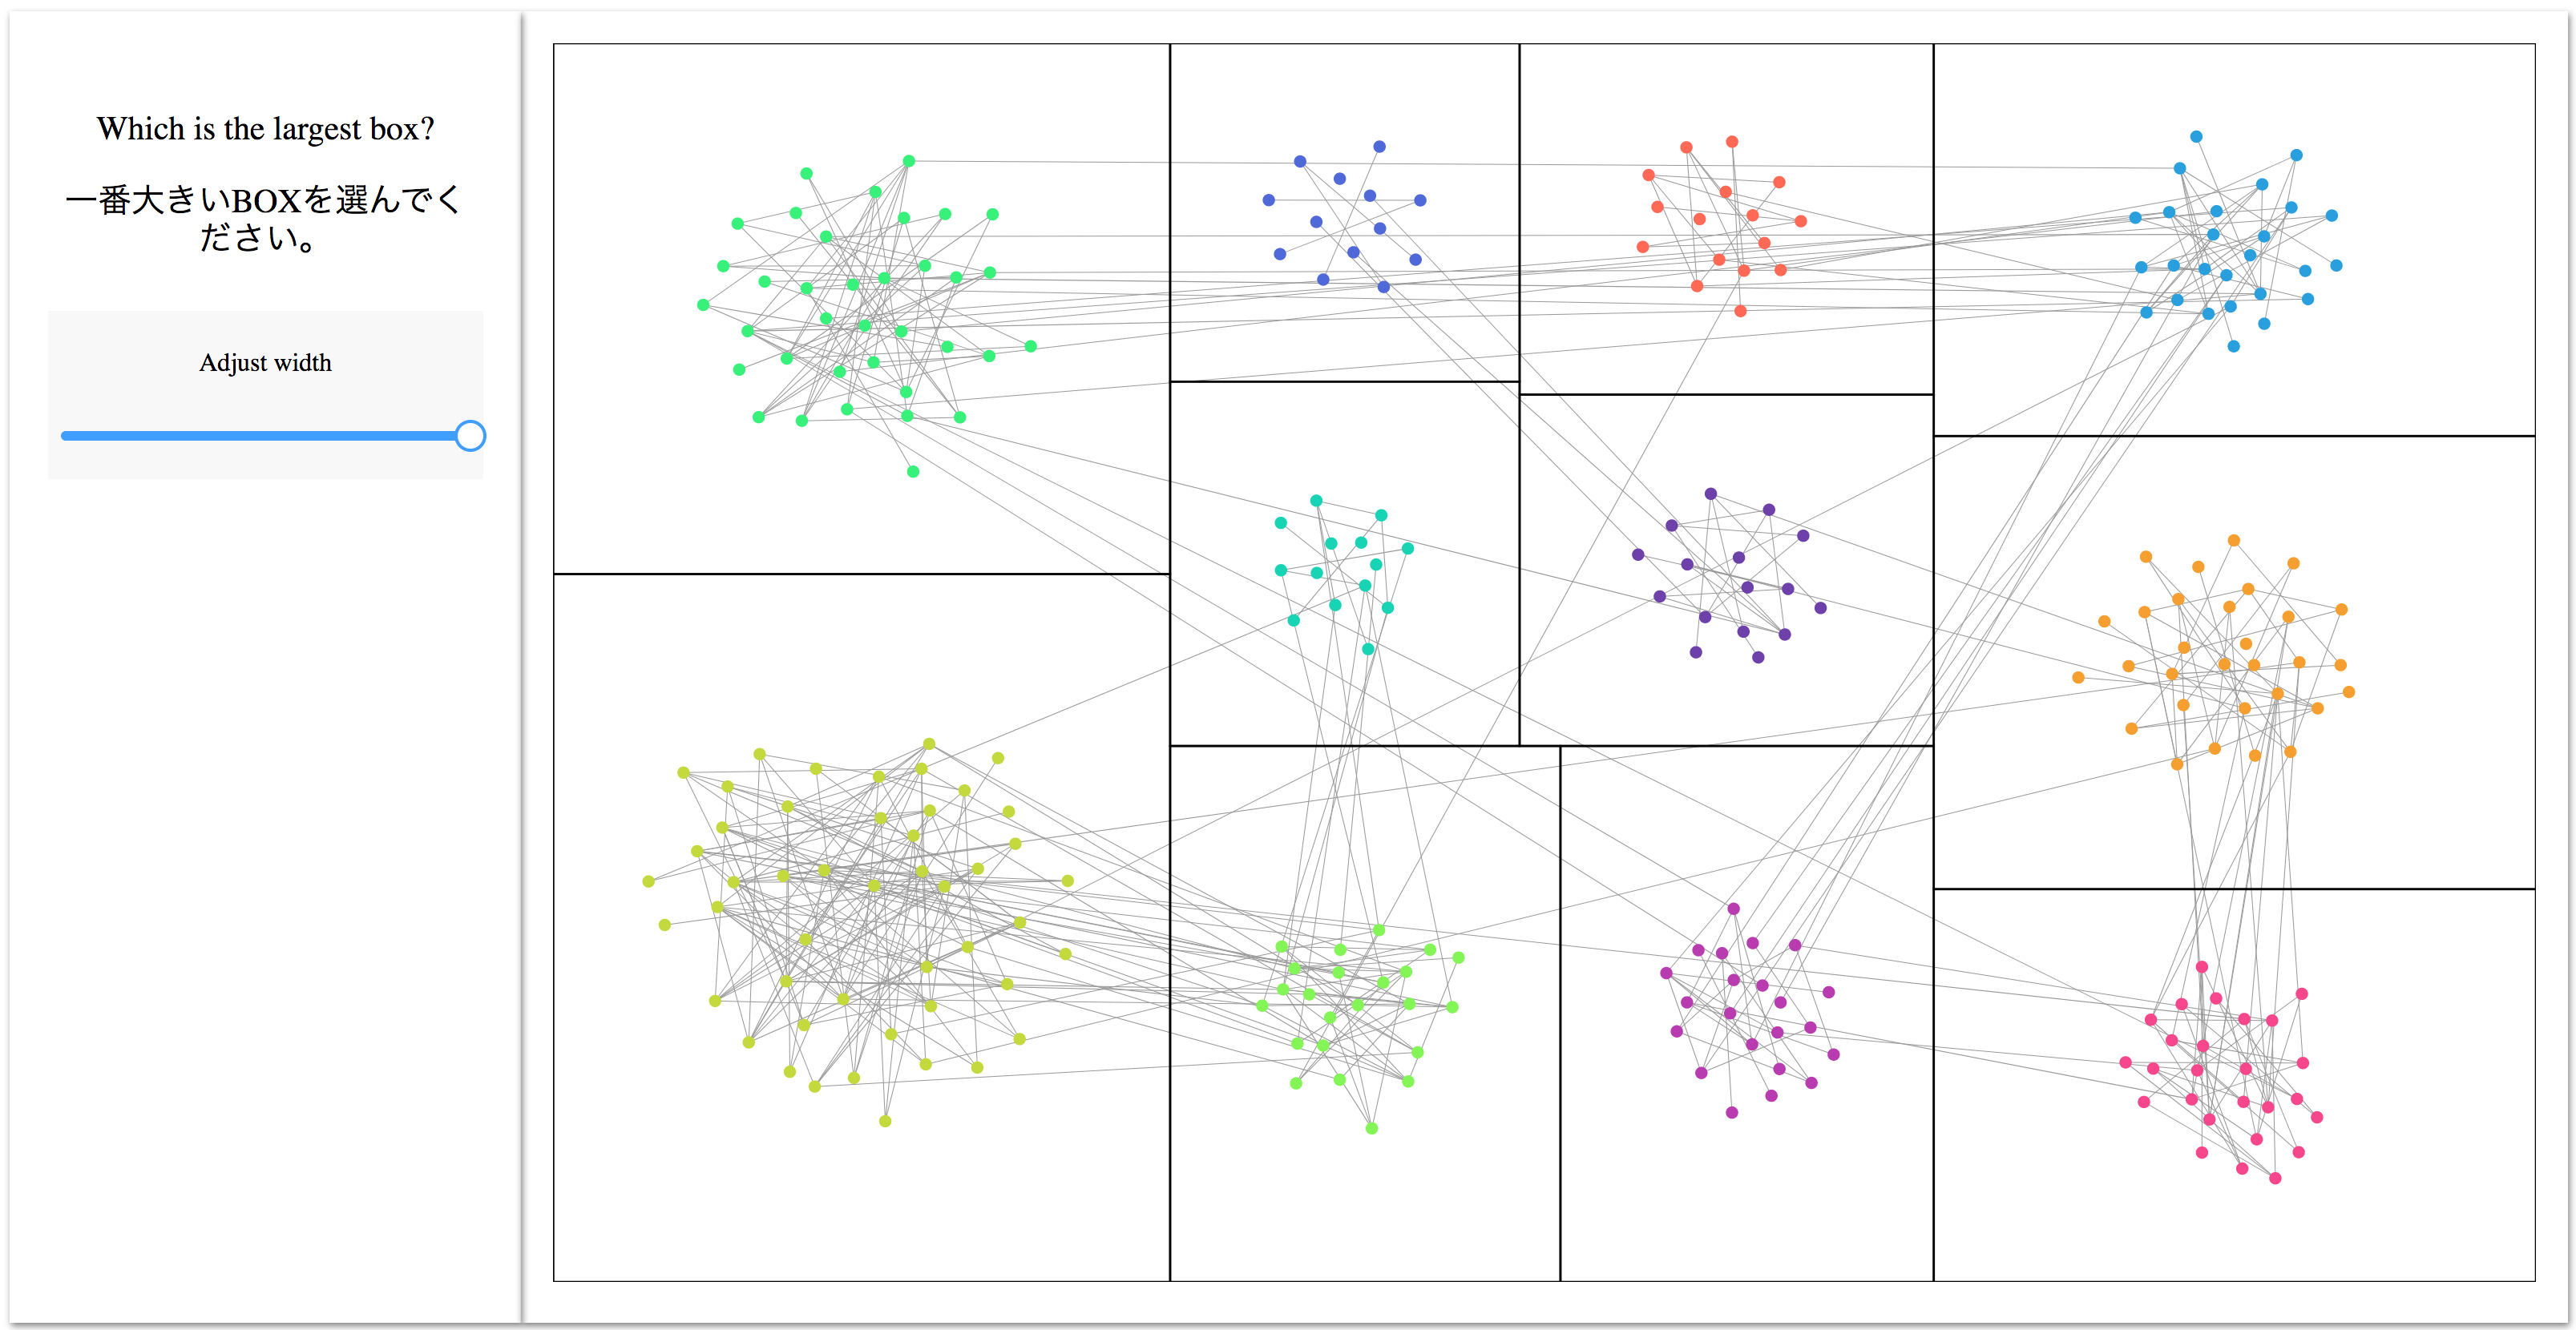
\includegraphics[width=0.45\textwidth]{pictures/screenshot.png}
    \caption{A screen shot of the actual experiment.}
    \label{screenShot}
  \end{center}
\end{figure}

We conducted this eye-tracking experiment in a room with artificial illumination and few objects.
The participants' mobile phones were switched off to reduce distractions during the experiments.
The eye movements were recorded using a Tobii Pro X3-120 eye-tracking system with an ASUS screen resolution of $2,018 \times 1,920$ pixels.
The participants sat in front of a display at a distance of 65~cm.
For the analysis software of the eye tracker, we utilized I-VT filter to determine whether a gaze was a fixation or a saccade, as described in \cite{olsen2012tobii}.

\subsection{Participants}

We used a within-subjects study design with 20 participants, all of whom were Japanese (eight women and 12 men).
Their average age was 20.8 years, with the youngest participant being 18 and the oldest participant being 24.
All were students at our university: four were studying engineering, whereas the other participants were students with various majors.
All participants had normal or corrected-to-normal color vision.
Each participant was compensated with the sum of 3,000 yen.
The experiment duration was 1.5--2 h, including the explanation and breaks.
We observed we had a critical problem of experiment system at 1 participants, so we excluded data from the participant and after all we collected data from 19 participants.

\section{Experimental Results}

\subsection{Task Results}
\label{taskResult}

In this subsection, we describe the results of the user experiments, excluding the eye-tracking data, which are discussed in the following subsection.
This subsection present the results of the statistical analysis of completion time and correctness of all tasks.
As the data were not normally distributed, we used non-parametric analysis methods for the analysis.
We conducted Friedman test to determine whether there was a significant difference, followed by post-hoc Wilcoxon signed rank test. In all cases, we used $0.05$ as a significance value.
Hereinafter, the statistical analyses of the results are discussed for each task separately, where we supposed that each layout has its advantages and disadvantages and that all tasks are independent.

\begin{figure*}[t]
  \begin{center}
    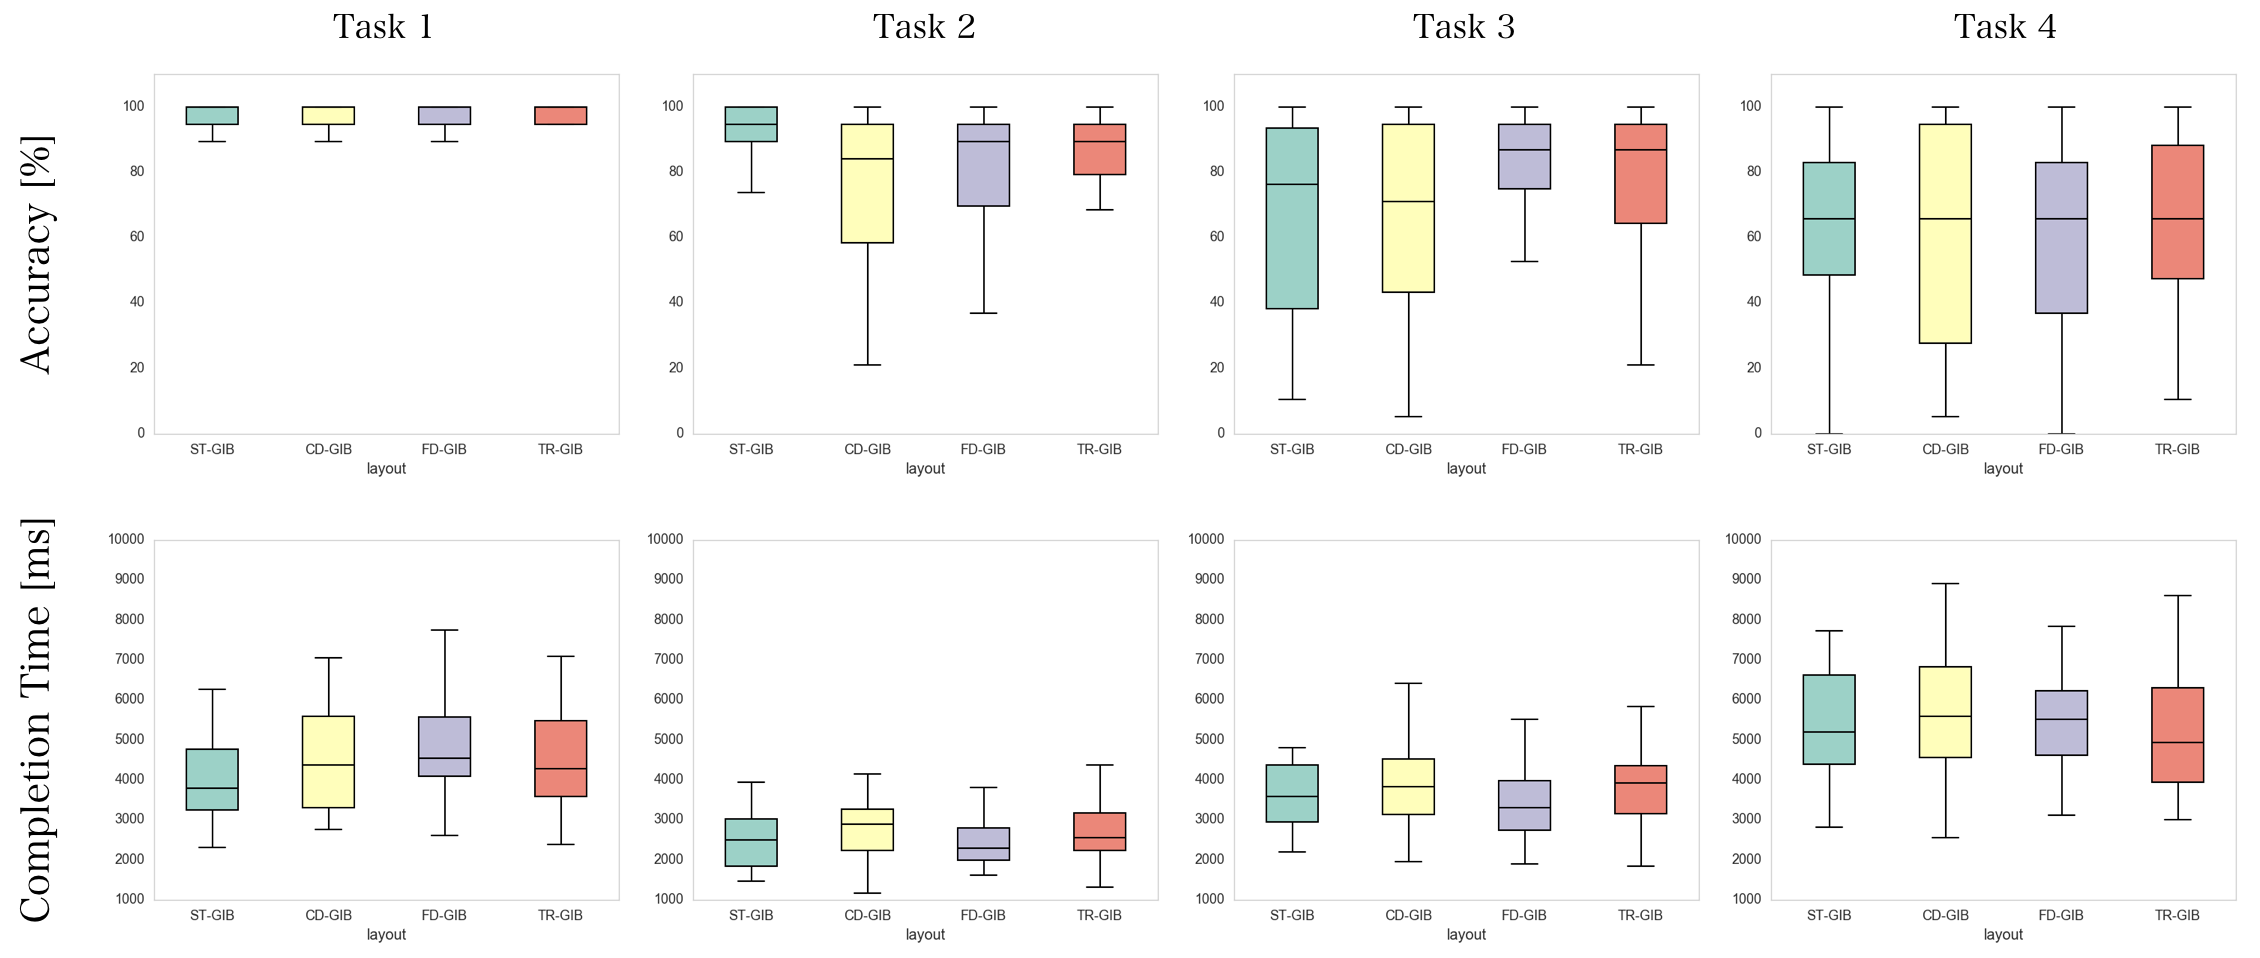
\includegraphics[width=1\textwidth]{pictures/results.png}
    \caption{Task results}
    \label{results}
  \end{center}
\end{figure*}

% \begin{table}[htb]
%   \begin{center}
%     \begin{tabular}{|c||c|c|c|c|} \hline
%       Layout & Task 1 & Task 2 & Task 3 & Task 4 \\ \hline \hline
%       ST-GIB & 98.1\% (3.987~s) & 89.6\% (2.535~s) & 67.4\% (3.606~s) & 62.8\% (5.387~s) \\ \hline
%       CD-GIB & 98.2\% (4.527~s) & 76.9\% (2.761~s) & 67.2\% (3.843~s) & 59.3\% (5.588~s)\\ \hline
%       FD-GIB & 96.7\% (4.919~s) & 82.9\% (2.427~s) & 78.8\% (3.382~s) & 59.3\% (5.518~s)\\ \hline
%       TR-GIB & 98.1\% (4.493~s) & 83.6\% (2.713~s) & 72.8\% (3.845~s) & 63.5\% (5.128~s)\\ \hline
%     \end{tabular}
%   \end{center}
%    \caption{Results of user study: mean accuracy (mean completion time)}
%   \label{user-result}
% \end{table}

{\bf Task 1:} The mean accuracy of all layouts was 97.7\% and the mean completion time was 4480 ms.
Fig.~\ref{results} shows the accuracies and completions times of 4 tasks. Friedman analysis gave a significant effect in completion time ($p < 0.001$) while no significant difference in the correctness.
The post-hoc Wilcoxon test found participants completed this task significantly earlier in ST-GIB and TR-GIB than in CD-GIB and FD-GIB ($p<0.001$), and also CD-GIB is faster than FD-GIB ($p<0.001$).

The time required for ST-GIB in this task was about 500 ms shorter than that of CD-GIB and TR-GIB, and 900 ms shorter than that of FD-GIB on average.
These results support the {\bf Hypothesis 1}.

{\bf Task 2:} ST-GIB was the best in accuracy with the mean accuracy 89.6\% and completion time 2526 ms, and FD-GIB had the fastest completion time with the mean accuracy 83.0 \% and completion time 2425 ms.
From the Friedman test, we observed significant differences in both correctness ($p<0.001$) and completion time ($p = 0.0025$) for this task.
The Wilcoxon test showed significant effectiveness of ST-GIB compared to all other layouts ($p<0.001$ for CD-GIB and FD-GIB; $p=0.0019$ for TR-GIB), and ineffectiveness of CD-GIB compared to all ($p<0.001$ for ST-GIB; $p=0.0041$ for FD-GIB; $p=0.0019$ for TR-GIB).

These results support the {\bf Hypothesis 2} and {\bf Hypothesis 3}. FD-GIB and TR-GIB were better than CD-GIB, but not as effective as ST-GIB, which place boxes in the order of their sizes.

{\bf Task 3:} FD-GIB resulted in the highest scores for both accuracy (78.8\%) and time (3383ms).
The Friedman test shows that there were significant differences in both of correctness and completion time ($p<0.001$).
According to the Wilcoxon test, FD-GIB was better than all layouts in terms of correctness ($p<0.001$ for ST-GIB and CD-GIB; $p=0.017$ for TR-GIB) and completion time ($p=0.007$ for ST-GIB; $p<0.001$ for CD-GIB and TR-GIB). It also show significant differences that participants resulted in more correctness in TR-GIB than ST-GIB ($p=0.039$) and CD-GIB ($p=0.049$), and participants finished Task 3 earlier in ST-GIB than CD-GIB ($p=0.014$) and TR-GIB ($p=0.014$).

These result refutes {\bf Hypothesis 4} and {\bf Hypothesis 5}: FD-GIB performed this task with the best accuracy and completion time. TR-GIB did not produce bad result but its accuracy was $6 \%$ lower and it required 500ms more to complete this task than than FD-GIB.

{\bf Task 4:} The mean accuracy of all layouts was 61.2\% and the mean completion time was 5405 ms.
The Friedman test shows there was a significnat difference in completion time ($p = 0.039$).
The Wilconxon test shows that participants reach thier answer 400 ms earlier in TR-GIB than in FD-GIB ($p=0.003$).

Therefore, {\bf Hypothesis 6} was not be confirmed. There was no difference in correctness, and TR-GIB was faster than the FD-GIB.


% \begin{table}[h]
%   \begin{center}
%     \begin{tabular}{|c||c|c|c|c|} \hline
%       & Task 1 & Task 2 & Task 3 & Task 4 \\ \hline \hline
%         Accuracy & 0.2377 & 2.579e$-7$ & 1.303e$-5$ & 0.3039 \\ \hline
%         Time & 9.009e$-16$ & 7.571e$-5$ & 4.706e$-5$ & 0.06275\\ \hline
%     \end{tabular}
%   \end{center}
%   \caption{P-values of ANOVA for accuracy and completion time}
%   \label{anova}
% \end{table}

\subsection{Eye-tracking Results}
In this section, we present the result of the eye tracking during the experiment and analyze that data against the hypotheses.
There are a lot of methods in eye-track analysis, and they are mainly allocated into two categories. One is the use of some computation measures, such as fixation duration or saccade length.
These measures let reseachers do statistical analyses because of their quantitativeness.
In this study, we often used the number of distractors before or after a participant gazed the correct answer for the first time as a measure.
The distractor mean the boxes except for the correct answer.
From here we call this measure before the first gaze as {\bf DB} and that of after the first gaze as {\bf DA}.

Another way is the visual analytics with some visualizations for eye-track data such as trajectory map, gaze heat map, or flow map.
There are also several studies providing guidlines about the analysis of eye tracking data \cite{andrienko2012visual,duchowski2007eye,kurzhals2014evaluating}. In order to analyze our data, we here aim to use these various methods properly. We would like to emphasize that our biggest purpose of usin eye tracking in this study is finding what element in a GIB layout helps or interrupts a task performance. Therefore, we describe our eye-tracking analysis based on our hypotheses with taking care of visual attributes in a GIB graph in this section.

{\bf Hypothesis 1:} This hypothesis could be confirmed by our experiment where ST-GIB achieved the highest accuracy. To verify our hypothesis, we computed an eye-track measure, gaze count. The computation result is shown in Table.~\ref{table-gazecount}. We conducted a statistical analysis using Friedman test as the section~\ref{taskResult}. We found there was a significant difference in the gaze counts of four GIB layouts ($p=0.040$). An post-hoc Wilcoxon test shows that ST-GIB did not have as many gaze counts as the others, where $p<0.001$. Fewer gaze counts indicate that there were a few recounting or some multiple counts at the same time, where participants might easily count the number of groups. Therefore, this eye track measure supports this hypothesis and we suppose the well-aligned boxes can help count the number.

{\bf Hypothesis 2:} ST-GIB achieve the best result in Task 2, which support this hypothesis. As shown in Table.~\ref{table-gazecount}, ST-GIB and FD-GIB did not require as many gazes as CD-GIB and TR-GIB. Friedman test found out there were significant differences of the number of gazes between ST-GIB and CD-GIB ($p=0.002$), between FD-GIB and CD-GIB ($p=0.002$), and between FD-GIB and TR-GIB ($p<0.001$). Another mesure, {\bf DB} shows a evidence of this hypothesis and is shown in Table~\ref{table-dist2}. We obserbed a significant difference in this measure ($p=0.009$), and this measure in ST-GIB was significantly fewer than in CD-GIB ($p=0.027$) and FD-GIB ($p=0.006$). This indicates that participants could easily reach the correct answer in ST-GIB, and we suppose this happened due to box sorted by size in it.

{\bf Hypothesis 3:} This hypothesis is supported by the result of Task 2 where CD-GIB was the worst in the correctness. In CD-GIB, it is inferred that some visual attributes prevented the participants from guessing the area visually.
We supposed this is due to the poor aspect ratio of box which might have counfused participants. We also found a clue to reveal what element in this layout interrupted the task performance in a gaze flow map shown in Fig.~\ref{task2flow}.
A gaze flow map represents the flow of fixation of the whole participants among boxe, and the width of each flow is proportional to the number of transitions of gaze from a box to another. We only visualize flows with more transitions than 3 \% of all. In the CD-GIB, candidate boxes for area comparison are sometimes placed apart, so the area comparison might be difficult.
Although TR-GIB had many gaze counts as CD-GIB, boxes that are candidates for area comparison are often located nearby since TR-GIB is what we reordered the tiles in ST-GIB, which shows that comparative work is relatively easy.
This figure also shows the difficulty of area comparison of boxes with poor aspect ratio: one of the three comparison target are horizontally logitudinal rectangle, and not easy to estimate its size visually. Therefore, we suppose the poor aspect ratio and the fact that boxes with close areas were placed apart resulted in low accuracy.

{\bf Hypothesis 4:} TR-GIB did not produce the best result in Task 3 and this hypothesis could not be confirmed, although this layout resulted in significantly with more correctness than ST-GIB and CD-GIB.
We suppose that the superiority of this layout lies in the small number of edge crossings and because intra-links are presented more clearly when there are fewer interferences by inter-links.
Table~\ref{table-dist3} also gave us a clue of this result.
TR-GIB and ST-GIB had the smallest numbers of {\bf DB}.
We observed a significant difference in this measure by Friedman test where $p<0.001$, and those of TR-GIB and ST-GIB are significantly smaller than those of CD-GIB and FD-GIB ($p<0.001$) in Wicoxon post-hoc test.
This means that participants did not required as many gaze to reach the correct box in TR-GIB and ST-GIB as CD-GIB and FD-GIB.
The boxes in TR-GIB and ST-GIB are well-arranged horizontally or vertically.
We suppose this aligned arrangement helped the participants to find the correct answer in Task 3 as well as in Task 2.
The task to find the box with the biggest / smallest number of intra-links tend to depend on detecting the box with biggedst / smallest area because a big box often have a lot of intra-links in both of our algorythm and the real world network.

Although ST-GIB was good at {\bf DB} above, it did not achieve high accuracy.
It was easy to gaze the correct answer as a candidate in Task 3 because of the well-aligned boxes, but the more edge-crossings might have made it challenging to compare the numbers of intra-edges.


{\bf Hypothesis 5:} Since FD-GIB acieved the best result in Task 3 in spite of its small boxes, this hypothesis was refuted. In FD-GIB there are not as many edge crossings as ST-GIB and CD-GIB, so it might have been easier to see the intra-links than them. Therefore, this result means the number of edge crossings should have been small but the box size did not have to be large in this task.
Table~\ref{table-dist3} showed that the participants required a large number of gaze counts before the first gaze at the correct answer, but the number of gaze points to the distractor after that was the smallest: we observed a significant difference ($p<0.001$) in {\bf DA} and post-hoc analysis provided us that {\bf DA} in FD-GIB is significantly smaller than the others ($p<0.001$ for ST-GIB and TR-GIB; $p=0.001$ for CD-GIB).
This result indecates that the participants took many gaze to gaze tha correct answer even as an candidate, but it required only a few gazes to make their dicisions after the first gaze.
We suppose this is because the participants estimate the number of intra-links visually ambiguously, and specifically they saw the links as a color.
Since we draw the edge with gray color, the number of edges could be seen as the density of the color representing the degree of aggregation.
Moreover, a box in FD-GIB is much smaller than that of the othres, so this trend might be particularly remarkable.
% Therefore, wa can say that FD-GIB would be effective to understand the abstract information about intra-relationships such as the number of intra-links, but for more concrete information another layout would be more effective such as TR-GIB.


{\bf Hypothesis 6:} We found no significant difference in the correctness of Task 4, and this hypothesis could not be confirmed.
Four layouts have the difference in their edge crossings, which is thought to affect the readability of a graph especially link information, but they did not make any difference.
In terms of the completion time, we observed that of TR-GIB was statistically shorter than that of FD-GIB.

Regarding the computation result in ref~\ref{comp-result}, we expected there would be a differences in the result as we observe differnces in the number of edge crossings and uniform edge length.
As a reason of this task's result, we found a gaze concentration in a trajectory map of this task as shown in Fig.~\ref{concent}.
The gaze data (pink line) are concentrated so as to overlap the bundle of inter-links, and we found this trend in many cases in this task.
Therefore, we suppose that participants were searching for the answer with this bundle as a clue.
Since certain group pairs in our graph have some strong connections, there were some link bundles.
Moreover, when we seach for a link bundle, a longer bundle which is undesirable for graph drawing often stands out visually than shorter one.
The long bundle of inter-links might have affected the result in this task, resulting in no difference in the correctness.

\begin{table}[htb]
  \begin{center}
   \caption{Mean gaze counts (stdev)}
    \begin{tabular}{|c|c|c|c|c|} \hline
      & ST-GIB & CD-GIB & FD-GIB & TR-GIB \\ \hline
      Task 1 & 12.5 (5.49) & 14.4 (6.79) & 15.6 (6.85) & 14.1 (6.31) \\ \hline
      Task 2 & 8.6 (5.11) & 9.2 (5.30) & 8.3 (4.04) & 9.1 (5.18) \\ \hline
    \end{tabular}
  \end{center}
  \label{table-gazecount}
\end{table}

\begin{table}[htb]
  \begin{center}
   \caption{The gaze count of distractors in Task 2 (stdev)}
    \begin{tabular}{|c|c|c|c|c|} \hline
      & ST-GIB & CD-GIB & FD-GIB & TR-GIB \\ \hline
      % Task 1 & 12.5 (5.49) & 14.4 (6.79) & 15.6 (6.85) & 14.1 (6.31) \\ \hline
      {\bf DB} & 3.6 (3.59) & 3.9 (3.67) & 4.1 (3.48) & 3.7 (3.06) \\ \hline
      {\bf DA}  & 2.84 (3.33) & 2.99 (3.67) & 4.1 (3.48) & 3.7 (3.06) \\ \hline
    \end{tabular}
  \end{center}
  \label{table-dist2}
\end{table}

\begin{table}[htb]
  \begin{center}
   \caption{The gaze count of distractors in Task 3 (stdev)}
    \begin{tabular}{|c|c|c|c|c|} \hline
      & ST-GIB & CD-GIB & FD-GIB & TR-GIB \\ \hline
      % Task 1 & 12.5 (5.49) & 14.4 (6.79) & 15.6 (6.85) & 14.1 (6.31) \\ \hline
      Before & 3.8 (4.64) & 5.1 (5.11) & 4.8 (4.38) & 3.8 (4.48) \\ \hline
      After  & 4.8 (4.65) & 4.8 (4.84) & 3.7 (4.27) & 5.3 (5.37) \\ \hline
    \end{tabular}
  \end{center}
  \label{table-dist3}
\end{table}

\begin{figure}
  \begin{center}
    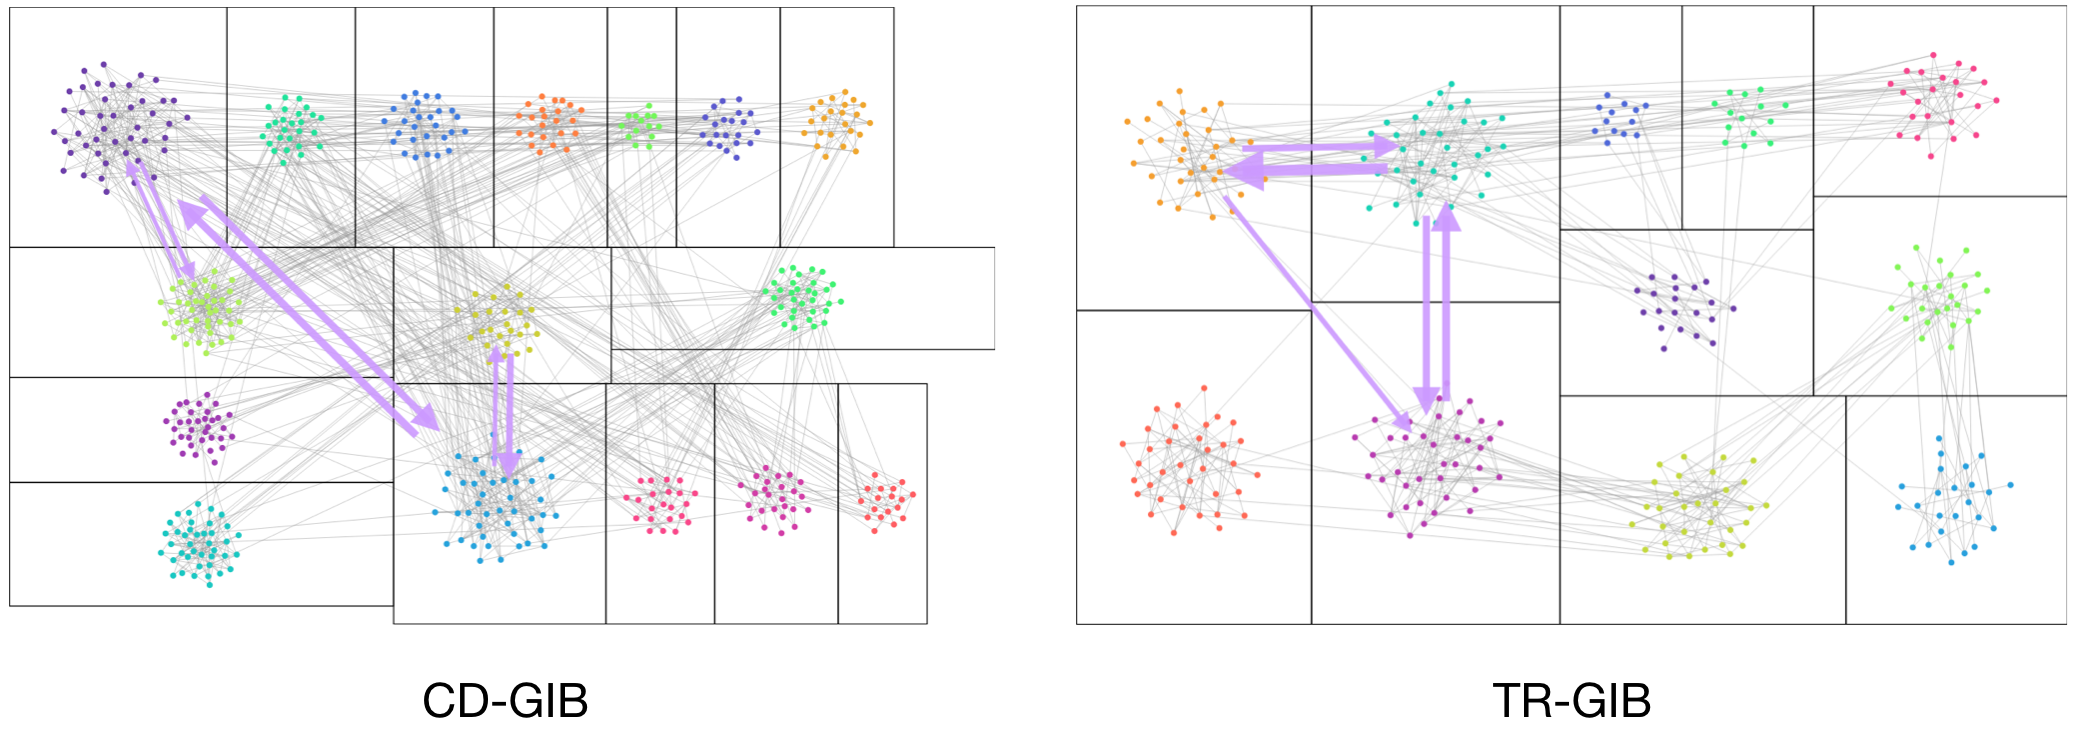
\includegraphics[width=0.48\textwidth]{pictures/cd-tr-in2.png}
    \caption{Flow map of CD-GIB and TR-GIB in Task 2}
    \label{task2flow}
  \end{center}
\end{figure}

\begin{figure}
  \begin{center}
    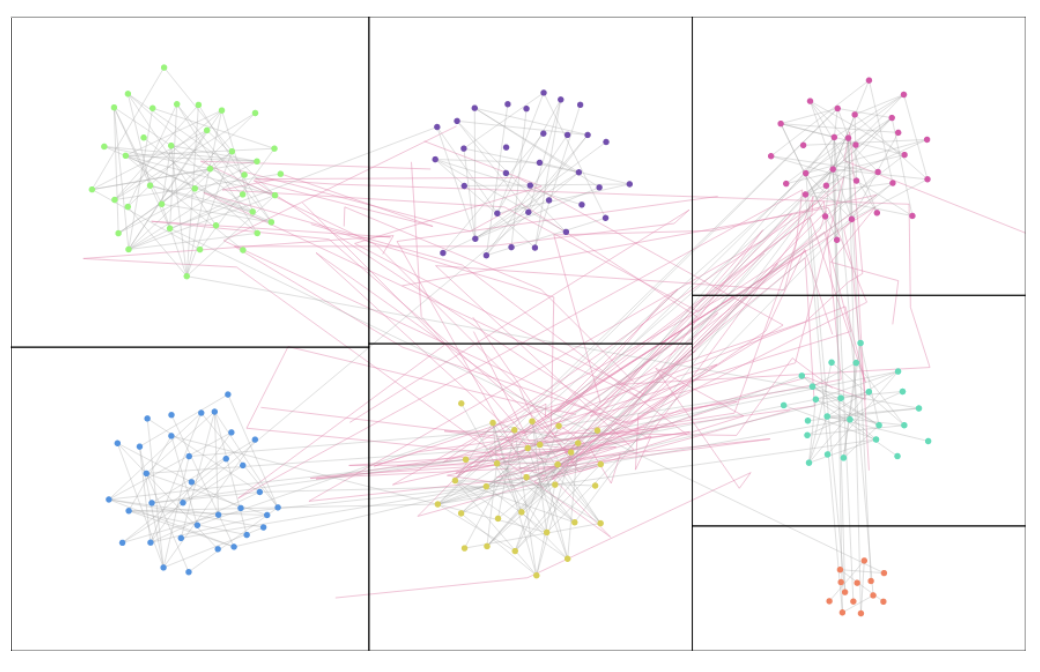
\includegraphics[width=0.3\textwidth]{pictures/concentration.png}
    \caption{A trajectory map in Task 4}
    \label{concent}
  \end{center}
\end{figure}

\section{Discussion}
We describe further discussion in this section, not only based on eye-track data. From here we discuss the experiment result along the four tasks.

{\bf Task 1:} This task was very simple with just counting the number of the boxes, but the four layouts made a statistical difference in the result at completion time.
Eye-track analysis gave us an clue that the well alignedness of ST-GIB was effective in this task.
We also found that FD-GIB required the most duration to detect the answer, where each box was smaller than the other layouts and pleced apart.
With respect to the Hypothesis 1, boxes should be well-arranged horizontally or vertically and presented with large size to count the number of them.

{\bf Task 2:} In this task, ST-GIB achieved the best result where boxes were placed in the order of area size and the aspect ratio of a box was not poor.
CD-GIB with bad aspect ratio of box was not accurate as the other layouts, while FD-GIB with the best aspect ratio was not so inaccurate and the fastest.
Therefore, a layout with good aspect ratio might be effective to detect the largest or smallest box.
We also reveal that the distance between the boxes as the candidates for comparison o the size is important.
Figure.~\ref{task2flow} shows that the boxes with similar size can be placed apart.
When these boxes are placed next to each other like ST-GIB and TR-GIB, the comparison process would be easier.

FD-GIB resulted in the shortest completion time, which indicates that the good aspect ratio of FD-GIB helped participants to compare the size between boxes.

{\bf Task 3:} Paricipants were required to detect a box with the most or fewest intra-links.
As the Hypothesis 4, we assumued that the number of edge crossings and was important in this task which indicates that it was challenging to discriminate an intra-link from an inter-link.
As a result, TR-GIB and FD-GIB which are the layout with fewer edge crossings had higher accuracies than the others.
A computational measure of eye tracking, namely {\bf DB} and {\bf DA}, gave us some evidences of this result.
TR-GIB had well-aligned boxes and the smallest {\bf DB}, which indicates that the easiness of the comparison of box size made it faster to reach the correct answer, and the fewwst number of edge crossings and the best uniform edge length helped to decide the answer correctly.
FD-GIB had the highest correctness and the smallest {\bf DA}.
With respect to the small boxes in FD-GIB in addition to this result, we suppose that participants could solve this task only by seeing thew color of a box which represent the dence of links.

We set this task to reveal which layout is the best for representing intra-links, From the studies of \cite{Vehlow2017VisualizingGS,saket2014group}, there is another task proper for this purporse, e.g., finding the vertex with the highest defree in a particular group.
This task require more concrete information than the ours, and FD-GIB might be not appropriate for this task because of its small boxes and poor uniform edge length.
We revealed the effectiveness of FD-GIB and TR-GIB in this task, but another task will be interesting.


{\bf Task 4:} We did not find any difference in the result of correctness, and TR-GIB did not require as much time to complete this task as FD-GIB.
Various factors can be considered as a cause of this, but in this study we were unable to find a difference with respect to the visibility of inter-links.

As a summary of the whole experiment, we found some trade-offs among each method for the type of user task.
ST-GIB achieved the best result in Task 1 and Task 2, while CD-GIB did not get remarkable result.
FD-GIB was not poor in all tasks, and it had the best result in Task 3.
Participants resulted in also not bad scores in all tasks in TR-GIB.

In the actual analysis of a real-world data, a graph must display links comprehensively.
In Task 3, FD-GIB and TR-GIB achieved good results which are not bad in other tasks, so we conclude that these two layouts are superior.
Since we found some trad-offs in the task result, so we recommend to use these properly for the user's purpose.
If a user aim to know the aggregate and abstract information of the graph, we suppose that FD-GIB is the best.
Participants could complete Task 2 and Task 3 the fastest in FD-GIB where a box is represented smaller, so this layout is suited for the quick and not so complecated task.

On the other hand TR-GIB can more display link information more concretely because of its good space efficiency.

By using these layouts properly depending on the purpose, more meaningful and effective analysis will be possible.


\section{Website of GIB}
As a part of our work, we provide a website which enable anyone to access the four GIB layouts easily: http://gib.jgs-hd.com.
Users can easily get the GIB layouts in the form of a bitmap or a svg imagefile with their own data.
It also enable further analysis.
Fig.~\ref{website} show an screen shot of the website.
There you can select any node by click, and then the node will be hilighted as well as the links connected to it.
You can see some detail informations of the node by put the mouse on it.
We hope this work can contributes many researchers by providing a lot of GIBs.

\begin{figure}
  \begin{center}
    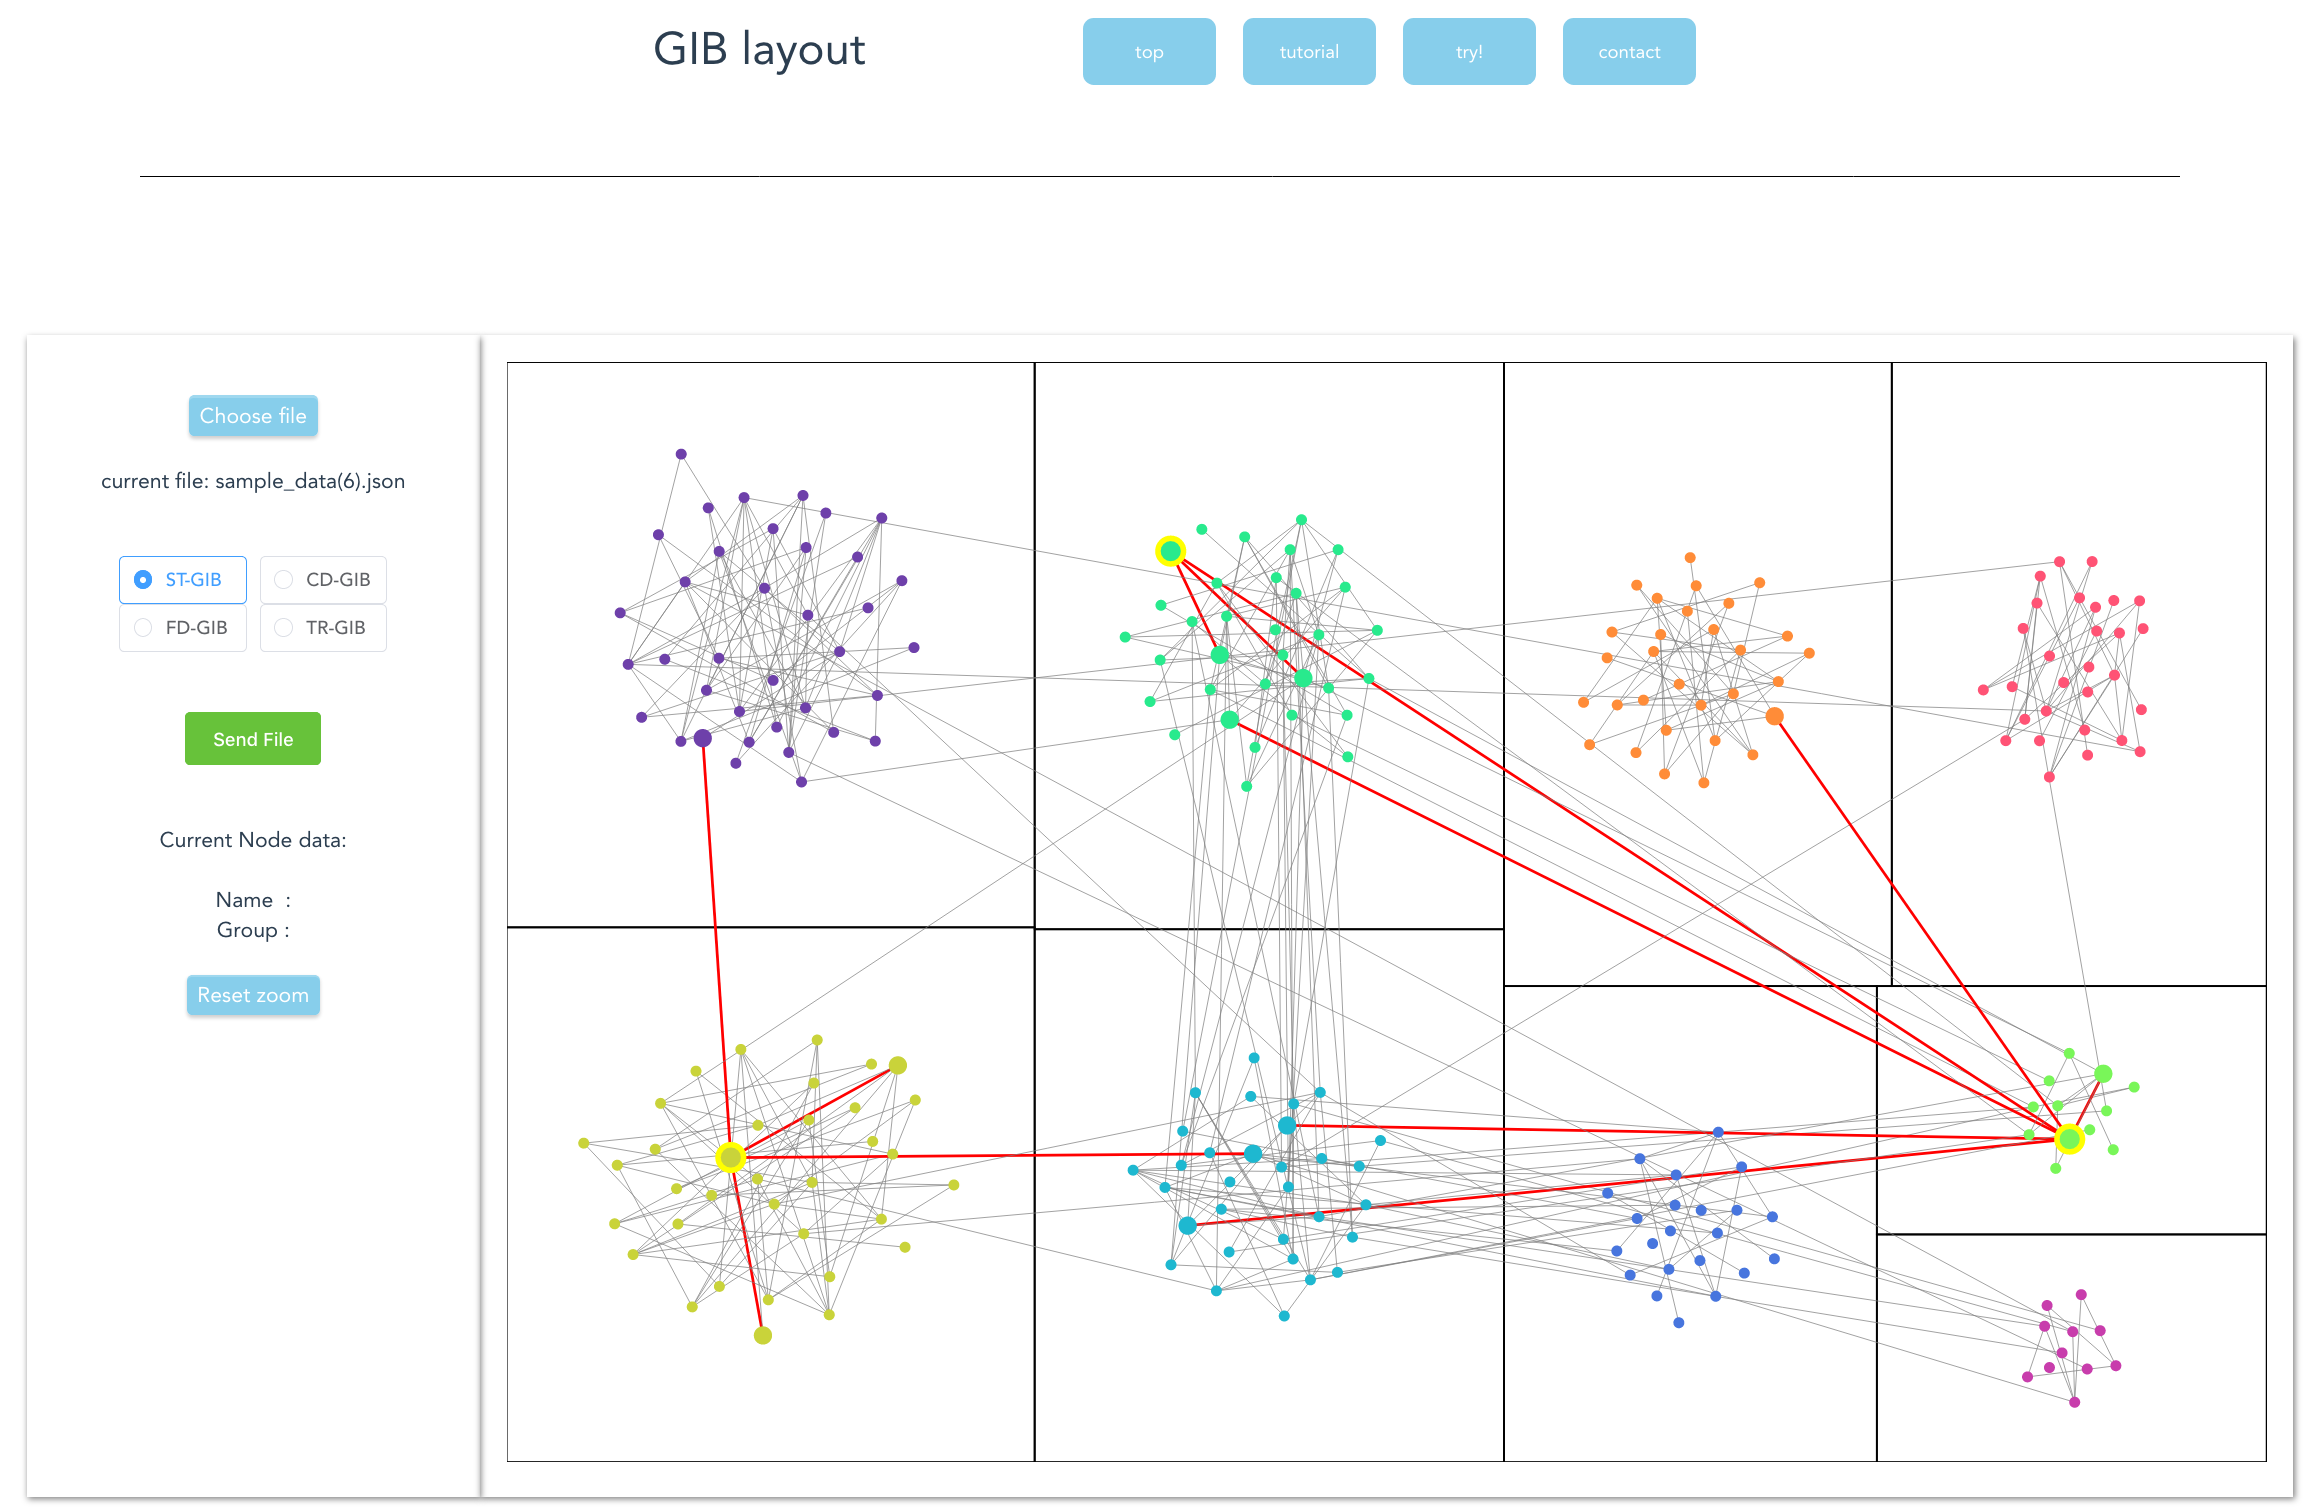
\includegraphics[width=0.48\textwidth]{pictures/website.png}
    \caption{An screen shot of the website we constructed.}
    \label{website}
  \end{center}
\end{figure}

%
\section{Conclusions}
%

In this study, we evaluated four GIB layouts by means of a user study with eye tracking.
We determined which layout is the best in four tasks and obtained evidence to support the results with eye tracking.
The best layouts were FD-GIB and TR-GIB which achieved higher performances in our tasks, with both layouts having their own advantages and disadvantages.
FD-GIB performed well in determining the number of links, a blurred information, whereas TR-GIB would be better in representing more concrete relationships, e.g., links between two specific nodes.
ST-GIB performed well in terms of understanding the size of each box; however, it was poor in interpreting links.

Eye-track data gave us some interesting clues to reveal what element in a visualization affect the task performance.
For example, well-alignedness in ST-GIB helped to count the number of groups.
Furthermore, the candidates for comparison were often placed apart in CD-GIB, which cause the difficulty of comparison and poor task performance.

We also provide a website that anyone can access the four GIB layout easily.
We hope this work can contribute meaningful discoveries to many reseachers.

Regarding the limitations of this work, other algorithms or methods could be used to generate random data, although we aimed to make them realistic.
In particular, we used only one set of parameters in the user study; thus, other cases would be of interest.
Additionally, there are several other ways of expressing nodes and edges and arranging nodes, which may influence the results.
We found that undesirable long edges were effective in task 4; therefore, another task may lead us to further results.

Our massive eye-tracking data could be used for further analysis as a future work.
Many methods that were not used in this study are available for dealing with eye-tracking data, which may lead to novel discoveries.

\section{Acknowledgments}
This work was supported by JST CREST Grant Number JPMJCR1511, Japan.


%\bibliographystyle{abbrv}
\bibliographystyle{abbrv-doi}
%\bibliographystyle{abbrv-doi-narrow}
%\bibliographystyle{abbrv-doi-hyperref}
%\bibliographystyle{abbrv-doi-hyperref-narrow}

\bibliography{template}
\end{document}
